\documentclass[12pt]{article}
\usepackage[OT1]{fontenc}
\usepackage[utf8]{inputenc}
\usepackage{kpfonts}
\usepackage{graphicx}
\usepackage[dvipsnames]{xcolor}
\usepackage{amsthm}
\usepackage[margin=1.25in]{geometry}
\usepackage[sf,bf,small,raggedright,compact]{titlesec}
\usepackage{hyperref}
\definecolor{linkblue}{named}{MidnightBlue}
\hypersetup{colorlinks=true, linkcolor=linkblue,  anchorcolor=linkblue,
        citecolor=linkblue, filecolor=linkblue, menucolor=linkblue,
        urlcolor=linkblue}
\usepackage[capitalize]{cleveref}
\usepackage{paralist}
\usepackage[longnamesfirst,numbers,sort&compress]{natbib}
% \usepackage[normalem]{ulem}


\usepackage{listings,newtxtt}
\lstset{basicstyle=\ttfamily, keywordstyle=\bfseries}


\newcommand{\pref}[1]{(P\ref{#1})}
\setlength{\parskip}{1ex}

\newtheorem{thm}{Theorem}
\newtheorem{obs}{Observation}
\newtheorem{lem}{Lemma}
\crefname{lem}{Lemma}{Lemmata}
\newtheorem{cor}{Corollary}
\newtheorem{clm}{Claim}
\newenvironment{clmproof}{\noindent\emph{Proof of Claim:}}{\hfill{$\blacksquare$}\par}

\crefname{dm}{}{}
\creflabelformat{dm}{#2(DM#1)#3}
\crefname{dp}{}{}
\creflabelformat{dp}{#2(DP#1)#3}
\crefname{p}{}{}
\creflabelformat{p}{#2(#1)#3}
\crefname{bg}{}{}
\creflabelformat{bg}{#2[bg#1]#3}


\DeclareMathOperator{\corners}{\Gamma}
\DeclareMathOperator{\dist}{d}
\DeclareMathOperator{\pack}{pack}
\DeclareMathOperator{\hit}{hit}

\newcommand{\defin}[1]{\emph{\textcolor{Maroon}{#1}}}


\theoremstyle{definition}
\newtheorem{definition}{Definition}[section]
\newtheorem{observation}{Observation}

\newcommand{\pat}[1]{[\textcolor{red}{PM: #1}]}
\newcommand{\vida}[1]{[{\color{pink}VD: #1}]}
\newcommand{\saeed}[1]{[{\color{blue}SO: #1}]}
\newcommand{\hussein}[1]{[\textcolor{purple}{$H^2$: #1}]}

\title{Connected Dominating Sets in Triangulations}
\author{Prosenjit Bose \and Vida Dujmović \and Hussein Houdrouge \and Pat Morin \and Saeed Odak}
% \date{}



\begin{document}

\maketitle

\begin{abstract}
  We show that every $n$-vertex triangulation has a connected dominating set of size at most $10n/21$.  Equivalently, every $n$ vertex triangulation has a spanning tree with at least $11n/21$ leaves. Prior to the current work, the best known bounds were $2n/3$ and $n/3$, respectively. (In the special case of Hamiltonian triangulations the previous bounds were $n/2$.)  As an application of this, we show that every $n$-vertex planar graph has a one-bend non-crossing drawing in which some set of at least $11n/21$ vertices is drawn on the $x$-axis.
\end{abstract}

% \vida{Note that if all the vertices of G are on a line then no edge in a 1-bend drawing crosses the line and thus G is subhamiltonian. Since not all planar graphs are subhamiltonian, that implies that the tight bound for the drawings above is strictly less than n. I wonder how much smaller than n it has to be. Is it a fraction of n? Do we know anything about the side of the largest induced subhamiltonian graph in a planar triangulation? Whatever we have on that line induces a subhamiltonian planar graph. So basically the result above also says that each planar graph has induced subgraph of size at least 11n/21 that is subhamiltonian planar. Do not know if that is interesting. n/4 follows trivially from 4-colour theorem. n/2 follows from the fact that every other layer of BFS induced an outerplanar graph.

% In either case we should say that n is not possible (or even better if we know that c*n is not possible for some $c<1$)
% }

% \saeed{As far as I am aware, all we know is Goldner–Harary Graph (\url{https://en.wikipedia.org/wiki/Goldner–Harary_graph}) is the smallest triangulation that is not subhamiltonian. you can put 10/11 of the vertices on a line. so the trivial upper bound on the size of the one-bend collinear set is 10/11. It would be interesting if we could glue a lot of copies of this example nicely to get a better upper bound. We conjecture that the size of the connected dominating set is at most $\frac{n}{3}$.  \sout{I guess (might be wrong) that the size of the largest collinear set is also at most $\frac{2n}{3}$.}}

% \vida{what if we take many copies of that graph and add one dominating vertex adjacent to all the vertices on outer faces of GH graph. Did not think about this. It is the first thing that came to my mind}

% \pat{I added a discussion of the relationship with subhamiltonian graphs after the statement of Theorem 2.}

\section{Introduction}

A set $X$ of vertices in a graph $G$ is a \defin{dominating set} if each vertex of $G$ is in $X$ or adjacent to a vertex in $X$.  A dominating set $X$ of $G$ is \defin{connected} if the subgraph $G[X]$ of $G$ induced by $X$ is connected.  There is an enormous body of literature on dominating sets, and several books are devoted to the topic \cite{haynes.hedetniemi.ea:domination,haynes.hedetniemi.ea:topics}.  A typical result in the area is of the form: ``Every $n$-vertex graph in some family $\mathcal{G}$ of graphs has a (connected) dominating set of size at most $f(n)$.'' or ``For infinitely many $n$, there exists an $n$-vertex member of $\mathcal{G}$ with no (connected) dominating set of size less than $g(n)$.''

A \defin{triangulation} is an edge-maximal planar graph.  \citet{matheson.tarjan:dominating} proved that every $n$-vertex triangulation has a dominating set of size at most $n/3=0.33\overline{3}n$ and that there exists $n$-vertex triangulations with no dominating set of size less than $n/4=0.25n$. The gap between these upper and lower bounds stood for over $20$ years until a recent breakthrough by \citet{spacapan:domination} reduced the upper bound to $17n/53\approx 0.32075471698n$.  This was swiftly followed by an improvement to $2n/7\approx 0.2\overline{857142}n$ by \citet{christiansen.rotenberg.ea:triangulations}.

In the current paper, we consider connected dominating sets in triangulations.  An easy consequence of the proof used by \citet{matheson.tarjan:dominating} is that triangulations have connected dominating sets of size at most $2n/3=0.66\overline{6}n$.  A more general result, due to  \citet{kleitman.west:spanning} shows that graphs of minimum-degree $3$ in which each edge is included in a $3$-cycle have connected dominating set of size at most $2(n-5)/3<0.66\overline{6}n$.  \citet{kleitman.west:spanning} also show that graphs of minimum degree $4$ have connected dominating sets of size at most $(3n-8)/5<0.6n$. This result applies to triangulations of minimum degree $4$, which includes all $4$-connected triangulations.  The main result in this paper is the following:

\begin{thm}\label{main_result2}
  For every $n\ge 4$, every $n$-vertex triangulation $G$ has a connected dominating set $X$ of size at most $10n/21= 0.\overline{476190}n$.
\end{thm}

The proof of \cref{main_result2} is constructive and gives an $O(n)$ time algorithm for finding the set $X$.  As far as we know, the best lower bound for this problem is $n/3-2 < 0.33\overline{3} n$, obtained from any triangulation that contains $n/3$ vertex-disjoint pairwise-nested triangles $\Delta_1,\ldots,\Delta_{n/3}$.  In order to dominate $\Delta_1$, any dominating set must contain at least one vertex in $\Delta_1 \cup \Delta_2$. In order to dominate $\Delta_{n/3}$, any dominating set must contain a vertex in $\Delta_{n/3-1}\cup\Delta_{n/3}$.  In order to be connected, any connected dominating set must contain a vertex in each $\Delta_2,\ldots,\Delta_{n/3-1}$.

\saeed{we can force the structure between $\Delta_1$ and $\Delta_2$ s.t. we need 2 vertices from $\Delta_1 \cup \Delta_2$ in the dominating set}


The original motivation for this research was a graph drawing problem.  It is know that every $n$-vertex planar graph $G$ has a non-crossing drawing in the plane with edges of $G$ drawn as line segments and such that some set $Y$ of $\Omega(n^{1/2})$ vertices of $G$ are drawn on the $x$-axis \cite{bose.dujmovic:polynomial,dujmovic:utility}.  The set $Y$ is called a \defin{collinear set}.  For bounded-degree planar graphs, this result can be improved to $|Y|=\Omega(n^{0.8})$ \cite{dujmovic.morin:dual}.  Determining the supremum value of $\alpha$ such that every $n$-vertex planar graph has a collinear set of size $\Omega(n^{\alpha})$ remains a difficult open problem, but it is known that $\alpha < 1$ \cite{ravsky.verbitsky:collinear}.

We consider a relaxation of this problem in which the edges of the graph can be drawn as a polygonal path consisting of at most two line segments.  Such a drawing is called a \defin{$1$-bend} drawing of $G$.  A subset $Y$ of $V(G)$ is a \defin{$1$-bend collinear set} if $G$ has a $1$-bend drawing in which all vertices of $Y$ appear on the $x$-axis.  We show that, for any connected dominating set $X$ in a triangulation $G$, the set $Y:=V(G)\setminus X$ is a $1$-bend collinear set of $G$.  Combined with \cref{main_result2}, this gives:

\begin{thm}\label{one_bend_collinear}
  For every $n\ge 4$, every $n$-vertex planar graph has a $1$-bend collinear set of size at least $11n/21=0.\overline{523809}n$.
\end{thm}

Note that if all the vertices of $G$ are on the $x$-axis then no edge in a $1$-bend drawing of $G$ crosses the $x$-axis, so this one bend drawing is a $2$-page book-embedding of $G$. This implies that $G$ is a spanning subgraph of some Hamiltonian triangulation $G^+$.  The Goldner–Harary graph is an $11$-vertex triangulation that is not Hamiltonian. It follows that the graph $G$ obtained by taking $k$ vertex-disjoint copies of the Goldner-Harary graph has $n:=11k$ vertices and has no $1$-bend collinear set of size greater than $10k=10n/11=0.90\overline{90}n$.





\subsection{Related Work}

\pat{Add: \newline
results on edge-maximal outerplanar graphs --- implies $n/2$ bound for Hamiltonian planar graphs (including $4$-connected.) \newline
connected dominating sets in unit disc graphs \newline
$2$-bend collinear sets \newline
$15$-approximation for minimum connected dominating set in planar graphs \newline
}
\saeed{

For every $n \in \mathbb{N}$, Everett et al. \cite{DBLP:conf/gd/EverettLLW07} show that there exists a universal set $\mathcal{U}_n$ of $n$ distinct points in the plane such that every $n$-vertex planar graph admits a 1-bend drawing with vertices on the points of set $\mathcal{U}_n$. Furthermore, Giacomo et al. \cite{DBLP:journals/comgeo/GiacomoDLW05} demonstrate that for a linear ordering $L$ of vertices of a planar triangulation $G$ and strictly convex curve $\lambda$, there is a $1$-bend plane drawing of $G$ such that vertices of $G$ appear on $\lambda$ with the same order as in $L$.

With further relaxation on the drawing of the edges, de Fraysseix et al. \cite{DBLP:journals/combinatorica/FraysseixPP90} show that any set of $n$ points in the plane is a universal set for the 2-bend drawing of planar graphs. Furthermore, They show that the planar embedding problem of any $n$-vertex graph on an $n$ collinear points in $\mathbb{R}^2$ with at most one bend along each edge is NP-complete.
}

The remainder of this paper is organized as follows:  In \cref{strategy}, we describe the general strategy we use for finding connected dominating sets in triangulations.  In \cref{warm_up} we show that a simple version of this strategy can be used to obtain a connected dominating set of size at most $4n/7= 0.\overline{571428}n$, which is already better than the best known bounds for triangulations.  In \cref{full_result} we show that a more careful construction leads to a proof of \cref{main_result2}.  In \cref{one_bend}, we discuss the connection between connected dominating sets and one-bend collinear drawings that leads to \cref{one_bend_collinear}.

% \subsection{Related Work}
%
% \pat{Explain how Kleitman-West result gives $3n/4$.  Explain how Matheson-Tarjan gives $2n/3$. Mention results on connected dominating sets in maximal outerplanar graphs.  Talk about connected dominating sets in unit disk graphs.}


\section{The General Strategy}
\label{strategy}

For a graph $G$, let $|G|=|V(G)|$ denote the number of vertices of $G$.  A \defin{bridge} in a graph $G$ is an edge $e$ of $G$ such that $G-e$ has more connected components than $G$.  For a vertex $v\in G$, $N_G(v):=\{w\in V(G):vw\in E(G)\}$ is the \defin{open neighbourhood} of $v$ in $G$,  $N_G[v]:=N_G(v)\cup\{v\}$ is the \defin{closed neighbourhood} of $v$ in $G$.  For a vertex subset $S\subseteq V(G)$, $N_G[S]:=\bigcup_{v\in S} N_{G}[v]$ is the \defin{closed neighbourhood} of $S$ in $G$ and $N_G(S):=N_G[S]\setminus S$ is the \defin{open neighbourhood} of $S$ in $G$.  A set $X\subseteq V(G)$ \defin{dominates} a set $B\subseteq V(G)$ if $B\subseteq N_G[X]$.  Thus, $X$ is a dominating set of $G$ if and only if $X$ dominates $V(G)$.

A \defin{plane graph} is a graph equipped with a non-crossing embedding in $\mathbb{R}^2$.  A plane graph is \defin{outerplane} if all its vertices appear on the outer face.  A \defin{triangle} is a cycle of length $3$. A \defin{near-triangulation} is a plane graph whose outer face is bounded by a cycle and whose inner faces are all bounded by triangles.  A \defin{generalized near-triangulation} is a plane graph whose inner faces are bounded by triangles. Note that a generalized near triangulation may have multiple components, cut vertices, and bridges


For a plane graph $H$, we use the notation $B(H)$ to denote the vertex set of the outer face of $H$ and define $I(H):=V(H)\setminus B(H)$.  The vertices in $B(H)$ are \defin{boundary vertices} of $H$ and the vertices in $I(G)$ are \defin{inner vertices} of $H$. For any vertex $v$ of $H$, the \defin{inner neighbourhood} of $v$ in $H$ is defined as $N_H^+(v):=N_H(v)\cap I(H)$, the vertices in $N^+_H(v)$ are \defin{inner neighbours} of $v$ in $H$, and $\deg^+_H(v)=|N^+_H(v)|$ is the \defin{inner degree} of $v$ in $H$.

Let $G$ be a triangulation.  Our procedure for constructing a connected dominating set $X$ begins with an incremental phase that eats away at the triangulation $G$ ``from the outside.'' The process of constructing $X$ is captured by the following definition:   A vertex subset $X\subseteq V(G)$ is \defin{outer-domatic} if it can be partitioned into non-empty subsets $\Delta_0,\Delta_1,\ldots,\Delta_{r-1}$ such that
\begin{compactenum}[(P1)]
    \item $\Delta_0\subseteq B(G)$; \label{outer_face}
    \item $\Delta_i\subseteq B(G-(\bigcup_{j=0}^{i-1}\Delta_j))$ for each $i\in\{1,\ldots,r-1\}$; and \label{incremental}
    \item $G-(\bigcup_{j=0}^{r-1}\Delta_j)$ is outerplanar. \label{outerplanar}
\end{compactenum}

\begin{lem}\label{outer_domatic}
    Let $G$ be a triangulation.  Then any outer-domatic $X\subseteq V(G)$ is a connected dominating set of $G$.
\end{lem}

\begin{proof}
  Suppose $X$ is outer-domatic and let $\Delta_0,\ldots,\Delta_{r-1}$ be the corresponding partition of $X$.  For each $i\in\{1,\ldots,r\}$, let $X_i:=\bigcup_{j=0}^{i-1} \Delta_i$.  First observe that, since $\Delta_0\subseteq B(G)$ is non-empty, $X_i$ contains at least one vertex of $B(G)$, for each $i\in\{1,\ldots,r\}$. We claim that,
  \begin{compactenum}[(P1)]\setcounter{enumi}{3}
    \item for each $i\in\{2,\ldots,r\}$ each vertex in $B(G-X_{i-1})$ is adjacent to some vertex in $X_{i-1}$. \label{adjacent}
  \end{compactenum}
  Indeed, for any $i\in\{2,\ldots,r\}$ and any vertex $v\in B(G-X_{i-1})$ is either in $B(G)$ or adjacent to a vertex in $X_{i-1}$. Even in the former case, (P1) ensures that $v$ is adjacent to a vertex in $X_1=\Delta_0\subseteq X_{i-1}$, because $G[B(G)]$ is a clique.

  We now prove, by induction on $i$, that $G[X_i]$ is connected, for each $i\in\{1,\ldots,r\}$.
  The fact that $G[B(G)]$ is a clique and \pref{outer_face} implies that $G[X_1]=G[\Delta_0]$ is connected. For each $i\in\{2,\ldots,r\}$, the assumption that $G[X_{i-1}]$ is connected, \pref{incremental}, and \pref{adjacent} then imply that $G[X_i]=G[X_{i-1}\cup\Delta_{i-1}]$ is connected.

  In particular $G[X_r]=G[X]$ is connected.  Finally, \pref{adjacent}, with $i=r$ and \pref{outerplanar} implies that $N_G(X_r)=B(G-X_r)=V(G-X_r)$, so $X_r=X$ is a dominating set of $G$.
\end{proof}

We will present two algorithms that grow a connected dominating in small batches $\Delta_0,\Delta_1,\ldots,\Delta_{r-2}$ that result in a sequence of sets $X_1,\ldots,X_{r-1}$ where $X_{i}=\bigcup_{j=0}^{i-1}\Delta_j$.  Each of these algorithms is unable to continue once they reach a point where each vertex in $B(G-X_i)$ has inner-degree at most $1$ in $G-X_i$.  We begin by studying the graphs that cause this to happen.

\subsection{Critical Graphs}

A generalized near-triangulation $H$ is \defin{critical} if $\deg^+_H(v)\le 1$ for each $v\in B(H)$. We that an inner face of $H[B(H)]$ is \defin{marked} if it contains an inner vertex of $H$.

\begin{figure}[htbp]
    \centering
    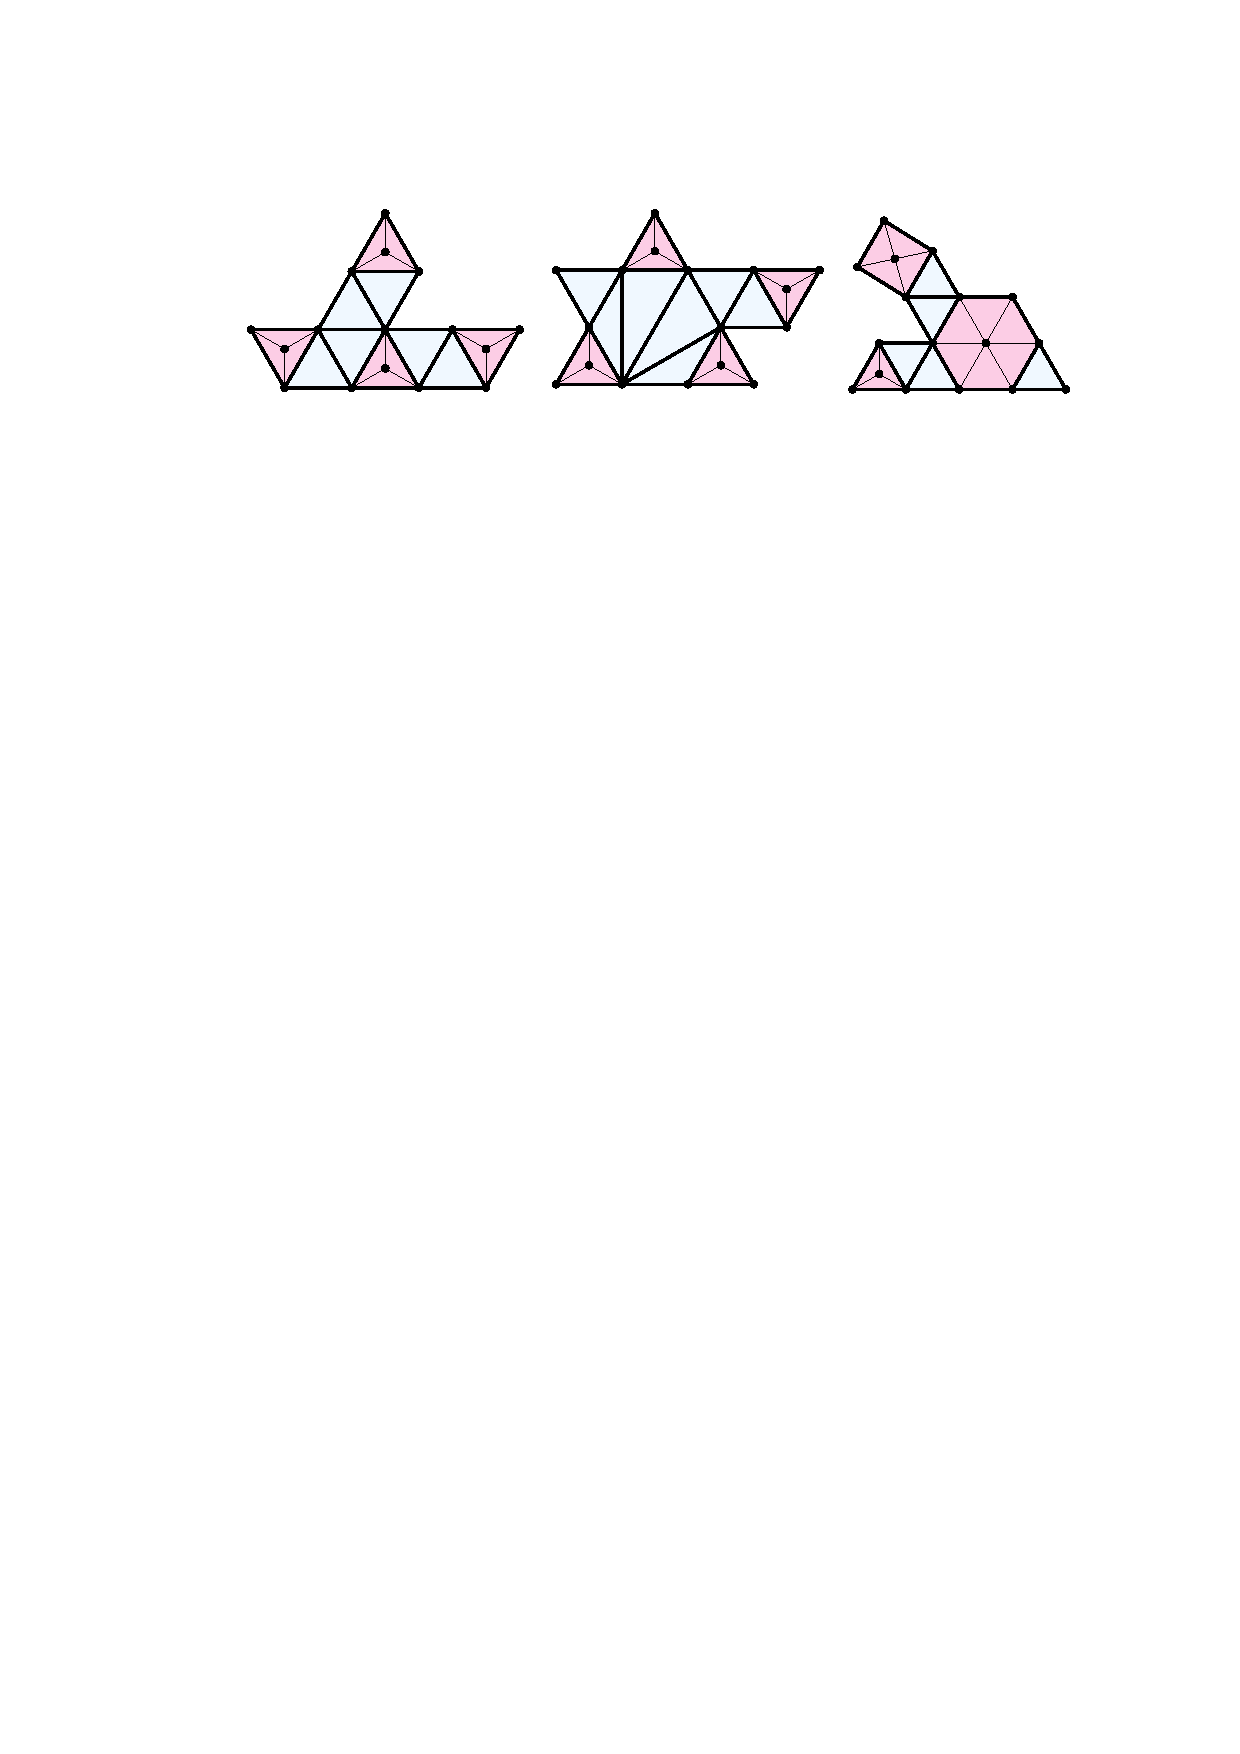
\includegraphics[page=1]{figs/critical}
    \caption{Some critical graphs.}
    \label{critical_fig}
\end{figure}


\begin{lem}\label{critical_structure}
    Let $H$ be a critical generalized near-triangulation. Then each $f$ face of $H[B(H)]$ contains at most one vertex of $I(H)$ and this vertex is adjacent to every vertex of $f$.
\end{lem}

\begin{proof}
  By definition, the graph $H[B]$ is outerplanar.  Consider some marked face $f$ of $H[B]$.  This face is marked because it contains at least one vertex in $I$.  Since $H$ is a triangulation, there is an edge $vx$ in $H$ with $v\in B$ on the boundary of $f$ and $x\in I$ in the interior of $f$. Since $H$ is a generalized near-triangulation and $x$ is an inner vertex of $H$, the edge $vx$ is on the boundary of two faces $vxv_1$ and $vxv_{k-1}$ of $H$ with $v_1\neq v_{k-1}$.  Since $\deg^+_H(v)=1$, each of $v_1$ and $v_{k-1}$ are in $B$.  By the same argument, $H$ contains a face $v_1xv_2$ with $v_2\in B$, $v_2\neq v$, and repeating this argument shows that $v,v_1,v_2,\ldots,v_{k-1}$ is the cycle in $H[B]$ that bounds $f$.  Therefore, $f$ contains exactly one vertex $x$ of $I$ and $x$ is adjacent to each vertex of $f$.
\end{proof}

\begin{lem}\label{base_case}
    Let $H$ be a critical generalized near-triangulation. Then $|B(H)|\ge 3|I(H)|$ and there exists $\Delta\subseteq B(H)$ of size at most $|I(H)|$ that dominates $I(H)$.
\end{lem}

\begin{proof}
  Let $B:=B(H)$ and $I:=I(H)$.  If $I$ is empty then the result is trivially true, by taking $X:=\emptyset$, so we now assume that $I$ is non-empty.  By \cref{critical_structure}, $H$ is formed from the outerplanar graph $H[B]$ by adding $|I|$ stars, one in the interior of each marked face of $H[B]$.  Furthermore, since $\deg_H^+(v)=1$ for each $v\in B$, each vertex of $H[B]$ is on the boundary of exactly one marked face.  For each vertex $w\in I$, the marked face that $f$ of $H[B]$ that contains $w$ has at least $3$ vertices, which do not belong to any other marked face. Therefore $|B|\ge 3|I|$ and by choosing one vertex from each marked face of $H[B]$ we obtain the desired set $\Delta$.
\end{proof}

% \begin{lem}\label{two_critical_helper}
%   Let $H$ be a biconnected critical generalized near-triangulation with at least two vertices.  Then $H[B(H)]$ has a proper $3$-colouring such that
%   \begin{compactenum}[(i)]
%     \item For each face $f$ of $H[B(H)]$ each colour appeas at least once;
%     \item For each marked face $f$ of $H[B(H)]$, there is a vertex $v_f$ whose colour is different from every other vertex in $f$.
%   \end{compactenum}
% \end{lem}
%
% \begin{proof}
%  The proof is by induction on the number $p$ of inner faces of $H[B(H)]$ with four or more vertices.  If $p=0$ then $H=H[B(H)]$ is an edge-maximal outerplanar graph and $H$ has a proper $3$-colouring that easily satisifies the conditions of the lemma.
%
%  Otherwise, let $f$ be a face of $H[B(H)]$ with four or more vertices. Then, by \cref{critical_structure}, the interior of $f$ contains a single vertex $x\in I(H)$ that is adjacent to every vertex in $f$.  Let $H'$
%
%  Otherwise, let $v$ be a vertex in $I(H)$ and let
%
%
%
%  If $|H|=3$ then, since $H$ is connected and bridgeless, $H$ is a cycle $vrw$. Then the conditions of the lemma are easily satisfied with $X_0:=\{v\}$, $X_1:=\{r\}$, and $X_2:=\{w\}$.  We now assume that $|H|\ge 3$.
%
%   % If $r$ has degree $1$, then let $r'$ be the unique neighbour of $r$ in $H$ and let $H':=H-r$.  Then $r'\in B(H')$ so we apply the inductive hypothesis on the instance $(H',r')$ to obtain sets $X_0',X_1',X_2'$ where $r'\in X_1'$, each of $X_1'$ and $X_2'$ dominate $V(H')$ and $X_0'$ dominates $V(H')\setminus \{r'\}$. Then we take $X_0:=X_{2}'$, $X_1:=X_0'\cup\{r'\}$ and $X_2:=X_1'$.  Then $X_1$ dominates $V(H)$ since $X_0'$ dominates $V(H)\setminus\{r,r'\}$ and $N_H[r]=\{r,r'\}$. Since $r'\in X_1'$, $X_2$ also dominates $V(H)$. The final set $X_0=X_2'$ dominates $V(H')=V(H)\setminus\{r\}$, as required.
%
%   If $r$ is a cut vertex of $H$, then $H-r$ has $k\ge 2$ components $C_1,\ldots,C_k$. For each $i\in\{1,\ldots,k\}$, let $H_i:=H[V(C_i)\cup\{r\}]$ and observe that $r\in B(H_i)$.  For each $i\in\{1,\ldots,k\}$,  we apply the inductive hypothesis on the instance $(H_i,r)$ to obtaine three sets $X_{i,0},X_{i,1},X_{i,2}$. Then, for each $i\in\{1,\ldots,k\}$,  $r\in X_{i,1}$, each of $X_{i,1}$ and $X_{i,2}$ dominate $V(H_i)$, and $X_{i,0}$ dominates $V(H_i)\setminus\{r\}$.  Then taking $X_0:=\bigcup_{i=1}^k X_{i,0}$,$X_1:=\bigcup_{i=1}^k X_{i,1}$, and $X_2:=\bigcup_{i=1}^k X_{i,2}$ gives the desired subsets of vertices.
%
%   If $\deg^+H(r)=1$ then let $f$ be the face of $H[B]$ that contains the single vertex $x\in N_H(r)\cap I$. Let $H'$ be the graph obtrained from $H$ by contracting the edge $rx$, creating a new vertex $r'$.  Then we apply the inductive hypothesis on the instance $(H',r')$ to obtain sets $X_0'$, $X_1'$, and $X_2'$ where $r'\in X_1'$, $X_1'$ and $X_2'$ dominate $V(H')$ and $X_0'$ dominates $V(H')\setminus\{r'\}$.
%
%
%   .  Without loss of generality, $r'\in X_1'$, each of $X_1'$ ad $X_2'$ dominate $V(H')$ and $X_0'$ dominates $V(H)\setminus\{r'
%   \}$.
%
%
%   Otherwise, suppose $r$ is not
%
%   Otherwise, $r$ is a vertex on the boundary of some inner face $f$ of $H[B]$.  If $f$ is a triangle $vrw$, then let $
%
%   If $f$ has four or more vertices then, by \cref{critical_structure}, $r$ is adjacent to an inner vertex $x$ contains in $f$.
%
%
%
%
%    each of which is a dominating set of $H$ and
% \end{proof}





\section{A Simple Algorithm}
\label{warm_up}

We start with the simplest possible greedy algorithm, that we call $\textsc{SimpleGreedy}(G)$, to choose $\Delta_0,\ldots,\Delta_{r-1}$.  Suppose we have already chosen $\Delta_0,\ldots,\Delta_{i-1}$ for some $i\ge 0$ and we now want to choose $\Delta_i$.  Let $X_i:=\bigcup_{j=0}^{i-1}\Delta_j$, let $G_i:=G-X_i$, and let $v_i$ be a vertex in $B(G_i)$ that maximizes $\deg^+_{G_i}(v_i)$.  During iteration $i\ge 0$, there are only two cases to consider:
\begin{compactenum}[{[}g1{]}]
    \item If $\deg^+_{G_i}(v_i)\ge 2$ then we set $\Delta_i\gets\{v_i\}$.
    \item If $\deg^+_{G_i}(v_i)\le 1$ for all $v\in G_i$ then $G_i$ is critical and this is the final step, so $r:=i+1$.  By \cref{base_case}, there exists $\Delta_i\subseteq B_i$ of size at most $|I_i|$ that dominates $I_i$. Then $X_r:=X_{r-1}\cup\Delta_{i}$ and we are done.
\end{compactenum}

\begin{thm}\label{simple_greedy}
  When applied to an $n$-vertex triangulation $G$,  $\textsc{SimpleGreedy}(G)$ produces a connected dominating set $X_r$ of size at most $(4n-9)/7$.
\end{thm}

\begin{proof}
By the choice of $\Delta_0,\ldots,\Delta_{r-1}$, $X_r$ is an outer-domatic subset of $V(G)$ so, by \cref{outer_domatic}, $X_r$ is a connected dominating set of $G$.  All that remains is to analyze the size of $X_r$.  For each $i\in\{1,\ldots,r\}$, let $D_i:=N_G[X_i]$ be the subset of $V(G)$ that is dominated by $X_i$, let $I_i:=V(G)\setminus D_i$ be the subset of $V(G)$ not dominated by $X_i$, and let $B_i:=N_G(I_i)$ be the vertices of $G$ that have at least one neighbour in each of $X_i$ and $I_i$.  We use the convention that $D_0:=B(G)$.

First observe that, for $i\in\{0,\ldots,r-2\}$, $|D_{i+1}|\ge |D_i|+\deg_{G_i}^+(v_i)$ since $D_{i+1}\supseteq D_i$ and $D_{i+1}$ contains the $\deg_{G_i}^+(v_i)$ inner neighbours of $v_i$ in $G_i$.  Therefore
\[
    |D_{r-1}| \ge |D_0| + \sum_{i=0}^{r-2} \deg_{G_i}^+(v_i) \ge 3 + \sum_{i=0}^{r-2} 2 =  2r+1 \enspace . \label{double_d}
\]
Since $D_{r-1}$ and $I_{r-1}$ partition $V(G)$,
\begin{equation}
  n = |D_{r-1}| + |I_{r-1}| \ge 2r+1 + |I_{r-1}|  \enspace . \label{c1}
\end{equation}

Since $X_{r-1}$ and $B_{r-1}$ are disjoint and $D_{r-1}\supseteq B_{r-1}\cup X_{r-1}$, we have $|D_{r-1}|\ge |X_{r-1}| + |B_{r-1}|=r-1+|B_{r-1}|$.  Therefore,
\begin{align}
    n & = |D_{r-1}| + |I_{r-1}| \ge r-1 + |B_{r-1}| + |I_{r-1}| = r-1 + |B_{r-1}| + |I_{r-1}| \notag
    \\
    & \ge r - 1 + 4|I_{r-1}| \enspace , \label{c2}
\end{align}
where the last inequality follows from \cref{base_case}.

The final dominating set $X_r$ has size $|X_r| = |X_{r-1}| + \Delta_{r-1} = r - 1 +|I_{r-1}|$, so the size of $|X_r|$ can be upper-bounded by maximizing $r-1+|I_{r-1}|$ subject to \cref{c1,c2}.  More precisely, by setting $x:=r$ and $y:=|I_{r-1}|$, the maximum size of $X_r$ is upper-bounded by the maximum value of $x-1+y$ subject to the constraints
\begin{align*}
x,y \ge 0 \\
  x - 1 + 4y & \le n \\
  2x + 1 + y & \le n
\end{align*}

% r\le (n+1-I_{r-1})/2$ and $r+4|I_{r-1}|\le n$.
This is an easy linear programming exercise and the maximum value of $X_{r}$ is obtained when $r=(3n-5)/7$ and $|I_{r-1}|=(n+3)/7$, which gives
$|X_r| \le (4n-9)/7$.
\end{proof}

\subsection{An $O(n)$ Time Implementation}

We note that the implementation of $\textsc{SimpleGreedy}(G)$ is even simpler than the definition given above.  Nothing special needs to be done for the critical graph $G_{r-1}$.  Repeatedly selecting a vertex of maximum innner-degree and removing it will produce a dominating set of size exactly $|I_{r-1}|$.  Thus, $\textsc{SimpleGreedy}(G)$ has a simple linear time implementation.  In this implementation, each vertex $v$ stores a value $d_v$ which is initially set to $\deg_G(v)$.  For the three vertices on the outer face of $G$, $d_v$ is initially set to $\deg_G(v)-2$.  In general, $d_v$ is kept updated so that it is always equal to the inner-degree of $v$ in $G_i$.

Besides the data structure used for representing the triangulation $G$, each vertex $v$ also participates in a doubly-linked list $L_{d_v}$  that stores all the vertices with the same $d_v$ value.  A global doubly-linked list $L$ then stores all the lists $L_d$ such that $L_d$ is non-empty, sorted by increasing order of $d$.   Extracting a vertex of maximum inner-degree can then be done in constant time and the total time spent moving vertices between different lists in $L$ is proportional to the number of edges of $G$. Thus, the entire algorithm can be implemented in $O(n)$ time.

\section{A Better Algorithm}
\label{full_result}

Next we devise an algorithm that produces a smaller connected dominating set than what $\textsc{SimpleGreedy}(G)$ can guarantee.  This involves a more careful analysis of the cases in which \textsc{SimpleGreedy} is forced to take a vertex $v_i$ with $\deg^+_{G_i}(v_i)=2$.  We will show that when this happens, one of the following two cases occurs:
\begin{compactenum}
  \item We can directly complete the dominating set $X_r=X_{i+1}$ by adding a set $\Delta_{r-1}=\Delta_i$ with at most $|G_i|/3$ additional vertices.
  \item We can add a pair of vertices $\{v_i,w_i\}$ that increase the size of the dominated set $D_{i+1}=N[X_{i+1}]$ by at least $5$ but only increase the size of the boundary set $B_{i+1}=B(G_{i+1})$ by at most $2$.
\end{compactenum}

% The commented out text below turns out to be completely bullshit
% \subsection{A Heuristic Analysis}
% Before diving into the details of how to make all this work, we present a heuristic analysis that explains why it gives a set $X$ of size at most $10n/21$.  Roughly speaking, Case~1 above implies that each vertex left in $G_{r-1}$ contributes $1/3$ to the size of the final dominating set $X_r$.  This implies that Case~2 above is more efficient than taking a vertex of inner-degree $3$.  Indeed, Case~1 adds two vertices $v_i$ and $y_i$ and increases the size of the boundary by $2$.  If the algorithm were to stop in the next iteration, these two new boundary vertices would contribute an additional $2/3$ to the size of $X_r$. Thus, Case~1 has a cost of $2+2/3=8/3$.  On the other hand, Case~1 decreases the number of undominated vertices by $5$, which is a measure of its progress.  On the other hand, choosing a vertex of inner-degree $3$ adds one vertex to $X$ and increases the size of the boundary by $2$, resulting in a cost of $1+2/3=5/3$ but only decreases the number of undominated vertices by $3$.  If we consider the ``progress over cost ratio'', the former case has a ratio of $5/(8/3)=15/8=1.875$ while the latter case has a ratio of $3/(5/3)=1.8$. We will formalize this informal argument by setting up a linear program to bound the maximum size of the final dominating set $X_r$. \pat{Maybe we can turn this informal argument into a potential function argument, instead?}

% In the end, optimizing this linear program shows that they hypothetical worst-case for the resulting algorithm is that it chooses inner-degree $3$ vertices for the first $r-1$ consecutive rounds, resulting in a graph $G_{r-1}$ with $|B(G_{r-1})|\approx 2r$ and $|I(G_{r-1})|\approx n-3r$, so $|G_{r-1}|\approx 2r+n-3r=n-r$.  The algorithm then finishes in Case~1, above, by taking a set $\Delta_{r-1}$ of size $|G_{r-1}|\approx (n-r)/3$.  This results in a dominating set $X_r$ of size roughly $r+(n-r)/3=n/3+(2/3)r$. This is a strictly increasing function of $r$, but the value of $r$ is constrained by the fact that $G_{r-1}$ has no vertices of inner-degree $3$, which implies that $|B(G_{r-1})|\ge |I(G_{r-1})|$.  This translates to the constraint $2r \le n-3r$ or $r \le n/5$.  Thus, the final dominating set has size at most $n/3 + (2/3)n/5=10n/21$.  We now make this heuristic analysis more formal.

\subsection{Dom-Minimal and Dom-Preserving Subgraphs}

We begin by identifying unnecessary vertices and edges that can appear in the graphs $G_1,\ldots,G_{r-1}$ during the construction of $X$.   We say that a near-triangulation $H$ is \defin{dom-minimal} if
\begin{compactenum}[({DM}1)]
    \item each vertex $v\in B(H)$ has $\deg^+_H(v)\ge 1$; and \label[dm]{bad_vertex}
    \item each edge $vw$ on the boundary of the outer face of $H$ is on the boundary an inner face $vwx$ of $H$ for some $x\in I(H)$. \label[dm]{bad_edge}
\end{compactenum}
We say that a generalized near-triangulation $H$ is \defin{dom-minimal} if each of its biconnected components are dom-minimal.

\begin{obs}\label{bridgeless}
    Any dom-minimal generalized near-triangulation $H$ is bridgeless.
\end{obs}

\begin{proof}
   If $vw$ is a bridge in $H$ then both $v$ and $w$ are in $B(H)$.  Since $vw$ is a bridge in $H$, there is no path $vxw$ in $H$ and hence no inner face $vwx$ in $H$. Thus $H$ does not satisfy \cref{bad_edge}.
\end{proof}

A subgraph $H'$ of a generalized near-triangulation $H$ is \defin{dom-preserving} if
\begin{compactenum}[({DP}1)]
  \item $B(H')\subseteq B(H)$; \label[dp]{boundary_subset}
  \item $N^+_{H'}(v)=N^+_H(v)$ for all $v\in B(H')$; \label[dp]{same_inner_neighbourhood}
  \item $I(H')=I(H)$; and \label[dp]{same_inner_vertices}
  \item $N_{H'}(v)=N_H(v)$ for all $v\in I(H)$. \label[dp]{same_neighbourhood}
\end{compactenum}

\begin{obs}
  Let $H$ be a generalized near-triangulation, let $H'$ be a dom-preserving subgraph of $H$, and let $\Delta$ be a subset of $V(H)$ that dominates $I(H)$.  Then $\Delta\cap V(H')$ dominates $I(H)$.
\end{obs}

\begin{proof}
  Each vertex $v\in I(H)=I(H')$ is adjacent to some vertex $w\in \Delta$.  Since $N_{H'}(v)=N_H(v)$, $w\in\Delta\cap V(H')$, so $v$ is dominated by $\Delta\cap V(H')$.  Since this is true for each $v\in I(H)=I(H')$, $\Delta\cap V(H')$ dominates $I(H)$.
\end{proof}

\begin{lem}\label{dom_minimal}
  For any generalized near-triangulation $H$, there exists a dom-preserving subgraph $H'$ of $H$ that is dom-minimal.
\end{lem}

\begin{proof}
  The proof is by induction on $|V(H)|+|E(H)|$.  If $H$ is already dom-minimal, then setting $H'=H$ satisfies the requirements of the lemma, so assume that $H$ is not dom-minimal.  It is straightforward to verify that the dom-preserving subgraph relationship is transitive, so if $H$ has a dom-preserving subgraph $H^*$ and $H^*$ has a dom-preserving subgraph $H'$ then $H'$ is a dom-preserving subgraph of $H$.  Therefore, it is sufficient to show the existence of a dom-preserving subgraph $H^*$ of $H$ with fewer edges or fewer vertices than $H$, and the inductive hypothesis provides the desired dom-minimal dom-preserving subgraph $H'$ of $H$.

  If $H$ contains a vertex $v\in B(H)$ with $\deg^+_H(v)=0$ then $H-v$ is a dom-preserving subgraph of $H$ with fewer vertices than $H$.  We now assume that $\deg^+_H(v)\ge 1$ for all $v\in B(H)$.  Since $H$ is not dom-minimal then $H$ contains a biconnected component $C$ that is not dom-minimal.
  \begin{compactenum}
    \item If there exists an edge $vw$ on the outer face of $C$ that is not incident to any inner face $vwx$ with $x\in I(C)$ then $B(H-vw)=B(H)$ and $I(H-vw)=I(H)$, and $H-vw$ is a is dom-preserving subgraph of $H$ that has fewer edges than $H$.

    \item If there exists a vertex $v\in B(C)$ with $\deg^+_C(v)=0$ then $v$ is incident to an edge $vw$ that is on the outer face of $C$ and on the outer face of $H$. Since $\deg^+_C(v)=0$, $vw$ is not incident to any inner face $vwx$ with $x\in I(C)$ and we can proceed as in the previous case. \qedhere
  \end{compactenum}
\end{proof}

% We say that a generalized near-triangulation $H$ is \defin{good} if
% \begin{compactenum}[(G1)]
%       \item $H$ is critical;
%       \item there exists $v\in B(H)$ with $\deg^+_H(v)\ge 3$; or
%       \item there exists distinct $v,w\in B(H)$ such that $\deg^+_H(v)=2$ and $N^+_H(w)\subseteq N^+_H(v)$.
% \end{compactenum}
%
% \begin{lem}\label{not_good}
%   Let $H$ be a dom-minimal generalized near-triangulation.  Then \begin{compactenum}[(i)]
%     \item $H$ is good or
%     \item $B(H)$ contains a vertex $v$ with $\deg^+_H(v)=2$ such that $G-v$ is good.
%   \end{compactenum}
% \end{lem}
%
% \begin{proof}
%   Since $H$ is dom-minimal, each vertex in $B(H)$ has inner-degree greater than $0$.  If some vertex in $B(H)$ has inner-degree at least $3$ then $H$ is good and there is nothing to prove, so we may assume that each vertex in $B(H)$ has inner-degree $1$ or $2$.  Since $H$ is not critical, at least one vertex in $B(H)$ has inner-degree $2$.  We distinguish between two cases, depending on whether $H$ is biconnected.
%
%   \pat{Updated here. The case where $H$ is biconnected needs a separate argument when $k=3$.}
%   If $H$ is biconnected then, since $H$ is bridgeless (by \cref{bridgeless}) the outer face of $C$ is a cycle $v_0,\ldots,v_{k-1}$ with $k\ge 3$. If there exists an edge $v_iv_{i+1}$ of this cycle with $\deg^+_H(v_i)=2$ and $\deg^+_H(v_{i+1})=1$ then $N_H^+(v_{i+1})\subset N_H^+(v_i)$ and $H$ is good, so we may assume that $\deg^+_H(v_i)=2$ for all $i\in\{0,\ldots,k-1\}$.
%   Let $v_i$ be a vertex in $B(H)$ such that $N_H(v_i)=N_H^+(v_i)\cup\{v_{i-1},v_{i+1}\}$.  Without loss of generality, assume $i=0$. Now consider the graph $H'=H-v_0$.  This graph contains two vertices, namely $v_{1}$ and $v_{k-1}$ with inner-degree $1$.  If $k\ge 4$, then $H'$ is good, because $\deg_{H'}^+(v_2)=2$ and $N^+_{H'}(v_1)\subseteq N^+_{H'}(v_2)$.  Otherwise, the outer face of $H'$ is a $4$-cycle $x_1,x_2,v_1,v_2$ and $N_H^+(v_1)\subseteq N_H^+(x_2)$ and $N_H^+(v_2)\subseteq N_H^+(x_1)$.  If $\deg^+_H(x_2)\ge 2$ or $\deg^+_H(x_1)\ge 2$ then $H'$ is good.  Otherwise all vertices in $B(H')$ have inner-degree at most $1$ in $H'$, so $H'$ is also good. Therefore $H$ contains a vertex $v:=v_0$ such that $H-v$ is good, as required.
%
%
%
%   If $H$ is not biconnected, then let $C$ be a biconnected component of $H$ that contains a single cut-vertex $v_0$ of $H$ (so $C$ is a leaf in the block-cut tree of $H$). Then $v_0$ is contained in a second biconnected component $C'\neq C$ of $H$. Since $H$ is dom-minimal, $\deg^+_{C}(v_0)\ge 1$ and $\deg^+_{C'}(v_0)\ge 1$, so $\deg^+_H(v)= 2$.
%
%   Since $C$ is biconnected, its outer face is bounded by a cycle $v_0,v_1,v_2,\ldots,v_{k-1}$.  If $\deg^+_C(v_1)=1$ then, since $H$ is dom-minimal, the edge $v_0v_1$ is on the boundary of an inner face $v_0v_1x$ with $x\in I(H)$.  Since $v_0$ is the only cut-vertex of $H$ in $C$, $N^+_H(v_1)=N^+_C(v_1)=\{x\}\subseteq N_H(v_0)$ and $\deg^+_H(v_0)=2$, so $H$ is good and there is nothing to prove.  We may therefore  assume that $\deg^+_C(v_1)=2$ and,  by the same reasoning, that $\deg^+_C(v_i)=2$ for each $i\in\{1,\ldots,k-1\}$.  (Otherwise, $N^+_H(v_i)\subseteq N^+_H(v_{i-1})$ and $\deg^+_H(v_{i-1})=2$ for some $i\in\{2,\ldots,k-1\}$ so $H$ is good.)
%
%   To summarize, so far we know that some vertex $x\in I(H)$ is in $N^+_H(v_0)$, $N^+_H(v_1)$, and $N^+_H(v_{k-1})$.  If $k=3$ then, since $H$ is dom-minimal, $H$ contains a face $v_1v_{k-1}y$ with $y\in I(H)$.  Since $\deg^+_H(v_1)=\deg^+_H(v_{k-1})=2$, $y\neq x$ and $N^+_H(v_1)=N^+_H(v_2)=\{x,y\}$. Again, this implies that $H$ is good.  We now assume that $k\ge 4$.
%
%   The edge $v_1v_2$ is on the boundary of a face $v_1v_2y$.  Since $\deg^+_H(v_1)=2$, $x\neq y$.  If $N^+_H(v_1)=N^+_H(v_2)=\{x,y\}$ then $v_1$ and $v_2$ satisfy (GM3), so $H$ is good.  Otherwise, consider the graph $H':=H-v_0$.  Then $\deg^+_{H'}(v_1)=1$, $\deg^+_{H'}(v_2)=2$, and $N_{H'}(v_1)\subseteq N_{H'}(v_2)$.   Therefore $H'$ is good, so $H$ contains a vertex $v=v_0$ of inner-degree $2$ such that $H-v$ is good.  This completes the proof.
% \end{proof}
%
%
% This gives variant of the $\textsc{SimpleGreedy}(G)$ that we call $\textsc{BetterGreedy}(G)$.  Suppose we have already chosen $\Delta_0,\ldots,\Delta_{i-1}$ for some $i\ge 0$ and we now want to choose $\Delta_i$.  Let $X_i:=\bigcup_{j=0}^{i-1}\Delta_j$, let $G_i$ be a dom-preserving subgraph of $G-X_i$ that is dom-minimal, and let $v_i$ be a vertex in $B(G_i)$ that maximizes $\deg^+_{G_i}(v_i)$.  During iteration $i\ge 0$, there are now four cases to consider:
% \begin{compactenum}
%     \item If $\deg^+_{G_i}(v_i)\ge 3$ then we set $\Delta_i\gets\{v_i\}$.
%     \item If there exists distinct $v_i,w\in B(H)$ such that $\deg^+_H(v_i)=2$ and $N^+_H(w)\subseteq N^+_H(v_i)$ then set $\Delta_i:=\{v_i\}$.
%     \item If $\deg^+_{G_i}(v_i)\le 1$ for all $v\in G_i$ then $G_i$ is critical and this is the final step, so $r:=i+1$.  By \cref{base_case}, there exists $\Delta_i\subseteq B_i$ of size at most $|I_i|$ that dominates $I_i$. Then $X_r:=X_{r-1}+\Delta_{i}$ and we are done.
%     \item Otherwise, $G_i$ is not good.  By \cref{not_good}, $G$ contains a vertex $v_i$ of inner-degree $2$ such that $G-v_i$ is good.  Set $\Delta_i:=\{v_i\}$.
% \end{compactenum}
%
% \begin{thm}\label{better_greedy}
%   When applied to an $n$-vertex triangulation $G$,  $\textsc{BetterGreedy}(G)$ produces a connected dominating set $X_r$ of size at most $(7n-14)/13$.
% \end{thm}
%
% \begin{proof}
%   Let $x_2$ be the number of times $\textsc{BetterGreedy}(G)$ falls into Case~4.
%   For each integer $t\ge 3$, let $x_t$ be the number of times $\textsc{BetterGreedy}(G)$ falls into case $1$ and chooses $v_i$ such that $\deg^+_{G_i}(v_i)=t$.  Let $z$ be the number of times $\textsc{BetterGreedy}(G)$ falls into Case~2.  From \cref{not_good}, we know that Case~4 never occurs during two consecutive iterations.  Therefore,
%   \begin{equation}
%       x_2 \le \sum_{t\ge 3}x_t + z + 1 \enspace .  \label{a1}
%   \end{equation}
%   The size of the dominated set $D_{r-1}$ is at least $|D_{r-1}| \ge 3 + \sum_{t\ge 2}tx_t + 2z$.
%   Since $|D_{r-1}|+|I_{r-1}|=n$,
%   \begin{equation}
%    3 + \sum_{t\ge 2}tx_t + 2z + I_{r-1} \le |D_{r-1}| + I_{r-1} \le n  \enspace . \label{a2}
%   \end{equation}
%   The of the boundary $B_{r-1}$ is at most $|B_{r-1}|\le 3+\sum_{t\ge 2}(t-1)x_t$.
%   By \cref{base_case},
%   \begin{equation}
%     3+\sum_{t\ge 2}(t-1)x_t \ge |B_{r-1}| \ge 3|I_{r-1}| \label{a3}
%   \end{equation}
%   The size of the final set $X_{r}$ is
%   \begin{equation}
%     |X_r| = \sum_{t\ge 2}x_t + z + |I_{r-1}| \enspace . \label{objective2}
%   \end{equation}
%   The unbounded number of variables $x_t$, $t\ge 2$ is problematic. We resolve this with the following claim:
%   \begin{clm}
%     In any assignment of non-negative values to $|I_{r-1}|$, $z$, and $x_2,x_3,\ldots$ that maximizes \cref{objective2} subject to \cref{a1,a2,a3}, $x_t=0$ for each $t\ge 3$.
%   \end{clm}
%   \begin{clmproof}
%      If $x_t = c >0$ for some $t\ge 3$, then we can set $x_t\gets 0$, $z\gets z+tc/2$, and $|I_{r-1}|\gets |I_{r-1}|-(t-1)c/3$.  This increases the value of \cref{objective2} by $tc/2-(t-1)c/3 =(t+2)c/6>0$.  The new values still satisfy \cref{a1} because the right hand side of \cref{a1} increases and the left hand side is unchanged.  The new values still satisfy \cref{a2} because the left hand side of \cref{a2} changes by $tc - 2tc/2 = 0$.  The new values still satisfy \cref{a3} because the left and right hand sides of \cref{a3} each decrease by $(t-1)c$.
%   \end{clmproof}
%   Therefore, \cref{a1,a2,a3} are three inequalities in three non-negative variables $x_2$, $z$, and $|I_{r-1}|$.  Maximizing \cref{objective2} subject to these constraints is an easy linear programming exercise that gives $x_2:=(3n-6)/13$, $z=(3n-19)/13$ and $I_{r-1}=(n+11)/13$, which gives $|X_r|= (7n+8)/13$.
% \end{proof}
%

% \section{The Best Algorithm}
% Let's see if we can beat $\textsc{BetterGreedy}(G)$.
% First, we need to rework our definition of dom-minimal a little bit:
%
% We say that a near-triangulation $H$ is \defin{dom-minimal} if
% \begin{compactenum}[({DM}1)]
%     \item there are no two vertices $v,w\in B(H)$ such that $N^+_H(w)\subseteq N^+_H(v)$; and
%     \item each edge $vw$ on the boundary of the outer face of $H$ is on the boundary of an inner face $vwx$ of $H$ for some $x\in I(H)$.
% \end{compactenum}
% We say that a generalized near-triangulation $H$ is \defin{dom-minimal} if each of its biconnected components are dom-minimal.
% Note that (DM1) implies that, unless $|H|=1$, each vertex $v\in B(H)$ has $\deg^+_H(v)\ge 1$.
%
% \Cref{bridgeless,dom_minimal} still hold under this new definition of dom-minimal.
%
% \pat{Did I really need to change the definition of dom-minimal?  Check.}


\subsection{Finding a $2$--$3$ Combo}

Note that the next two lemmas each consider a graph $H$ that is a near triangulation, not a generalized near-triangulation.

\begin{lem}\label{chord_incident}
  let $H$ be a dom-minimal near-triangulation and let $v_0$ be a vertex in $B(H)$ with $|N_H(v_0)\cap B(H)|\ge 3$.  Then $\deg^+_H(v_0)\ge 2$.  In other words, if $v_0$ is incident to a chord of the outerplane graph $H[B(H)]$, then $v_0$ is incident to at least $2$ inner vertices of $H$.
\end{lem}

\begin{figure}[htbp]
  \centering
  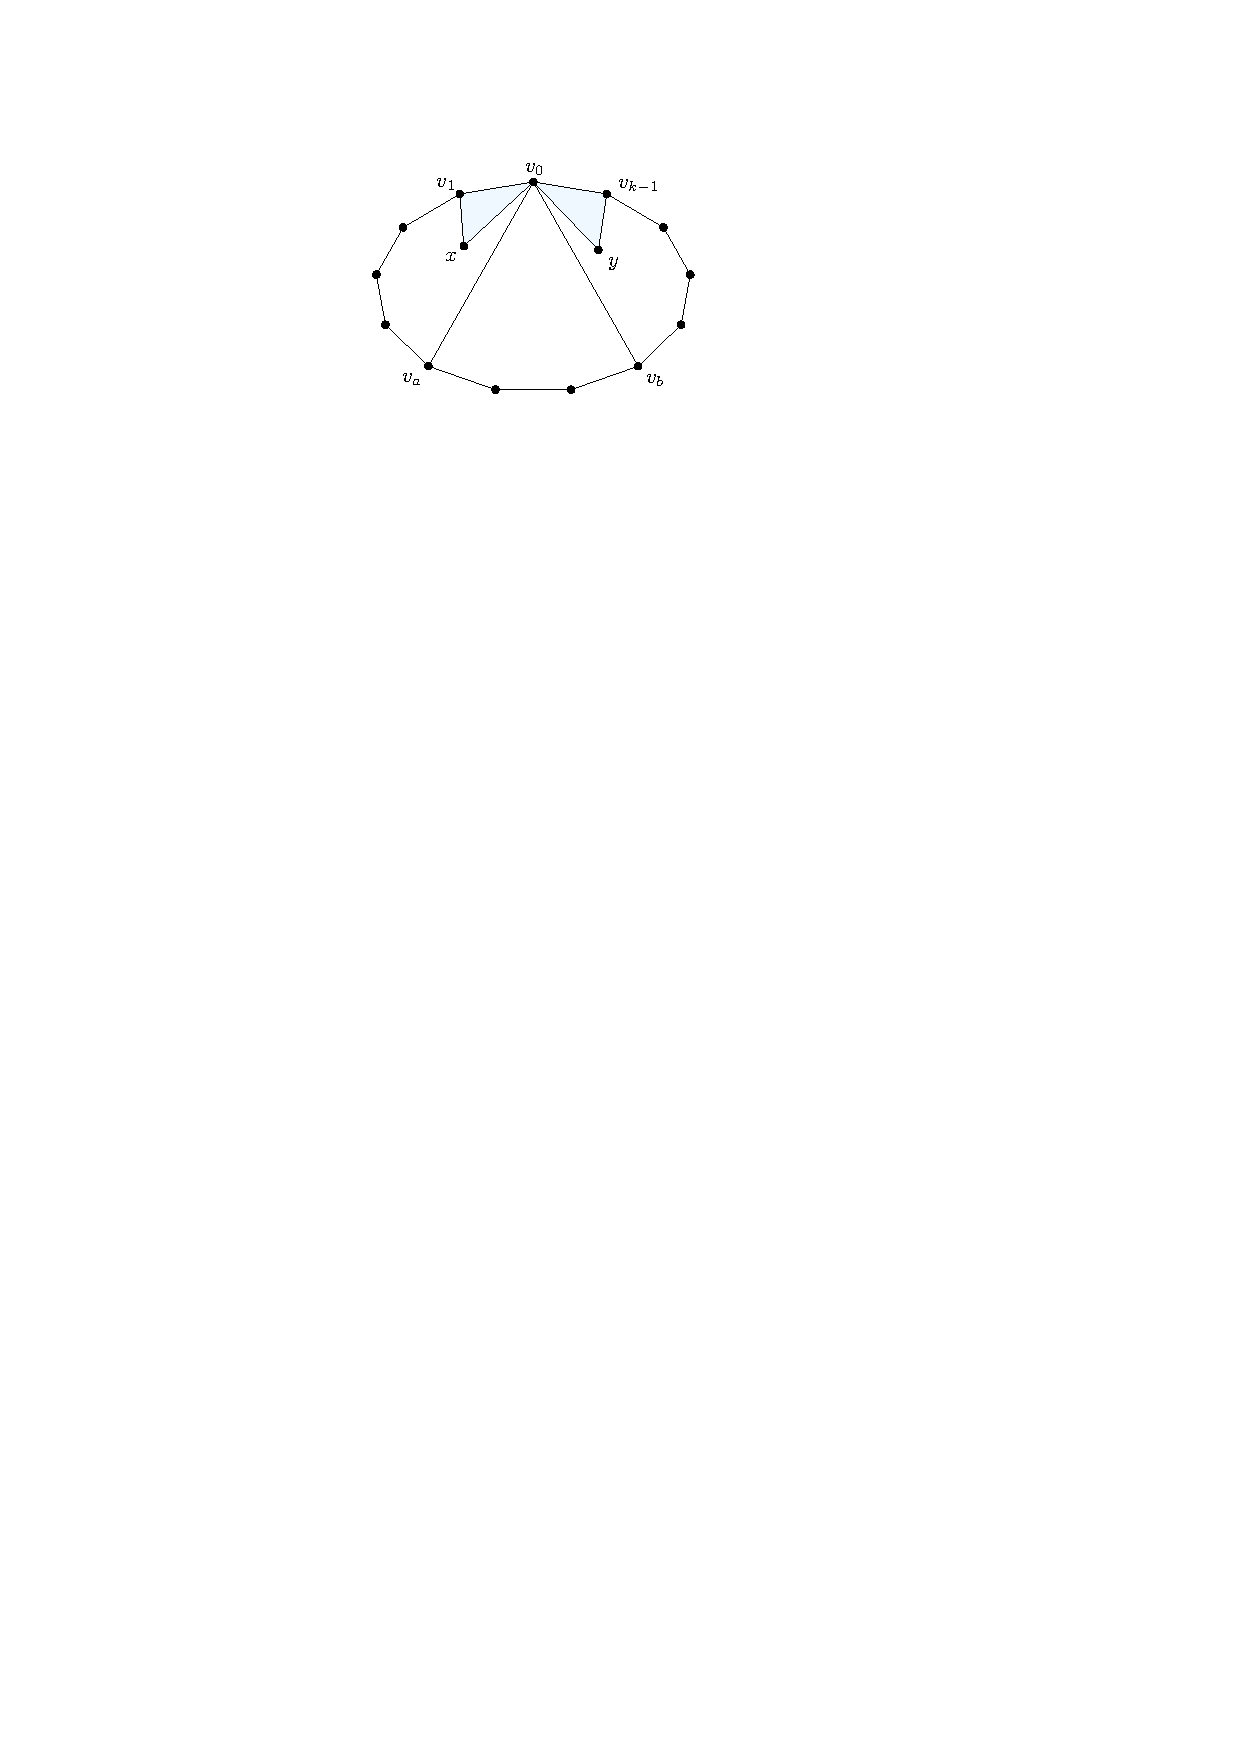
\includegraphics{figs/chord_incident}
  \caption{The proof of \cref{chord_incident}}
  \label{chord_incident_fig}
\end{figure}
\begin{proof}
  Refer to \cref{chord_incident_fig}
  Since $H$ is a near-triangulation its outer face is bounded by a cycle $v_0,\ldots,v_{k-1}$.  Let $a:=\min\{i\in\{2,\ldots,k-2\}:v_0v_i\in E(H)\}$ and $b:=\max\{i\in\{2,\ldots,k-2\}:v_0v_i\in E(H)\}$. (Possibly $a=b$, but both $a$ and $b$ are well-defined since $|N^+_H(v_0)|\ge 3$.)   Since $H$ is dom-minimal, the edge $v_0v_1$ is on the boundary of an inner face $v_0v_1x$ of $H$ where $x$ is an inner vertex of $H$.  Since $H$ is dom-minimal, the edge $v_{k-1}v_0$ is on the boundary of an inner face $v_{k-1}v_0y$ of $H$ where $y$ is an inner vertex of $H$.  Then $x$ is in the interior of the face of $H[B(H)]$ bounded by the cycle $v_0,v_1,\ldots,v_a$ and $y$ is in the interior of the face of $H[B(H)]$ bounded by the cycle $v_0,v_b,\ldots,v_{k-1}$.  Therefore, $x\neq y$ and $N^+_H(v_0)\supseteq\{x,y\}$ so $\deg^+_H(v_0)\ge 2$.
\end{proof}

\begin{lem}\label{degree_2_outer_neighbour}
  Let $H$ be a dom-minimal near-triangulation. Then either:
  \begin{compactenum}
    \item $H$ is outerplane;
    \item $H$ consists of a cycle on the vertices in $B(H)$ plus one dominant inner vertex $w$; or
    \item each vertex $w\in B(H-B(H))$ has a neighbour $v$ in $H$ with $\deg^+_H(v)\ge 2$.
  \end{compactenum}
\end{lem}

\begin{proof}
   If $H$ is outerplane then there is nothing to prove, so assume otherwise. Let $w$ be a vertex in $B(H-B(H))$. Since $w\not\in B(H)$, $w$ is an inner vertex of $H$. Consider the face $f:=v_0,\ldots,v_{k-1}$ of the outerplane graph $H[B(H)]$ that contains $w$. See \cref{degree_2_outer_neighbour_fig}.

   \begin{figure}[htbp]
     \centering
     \begin{tabular}{cc}
       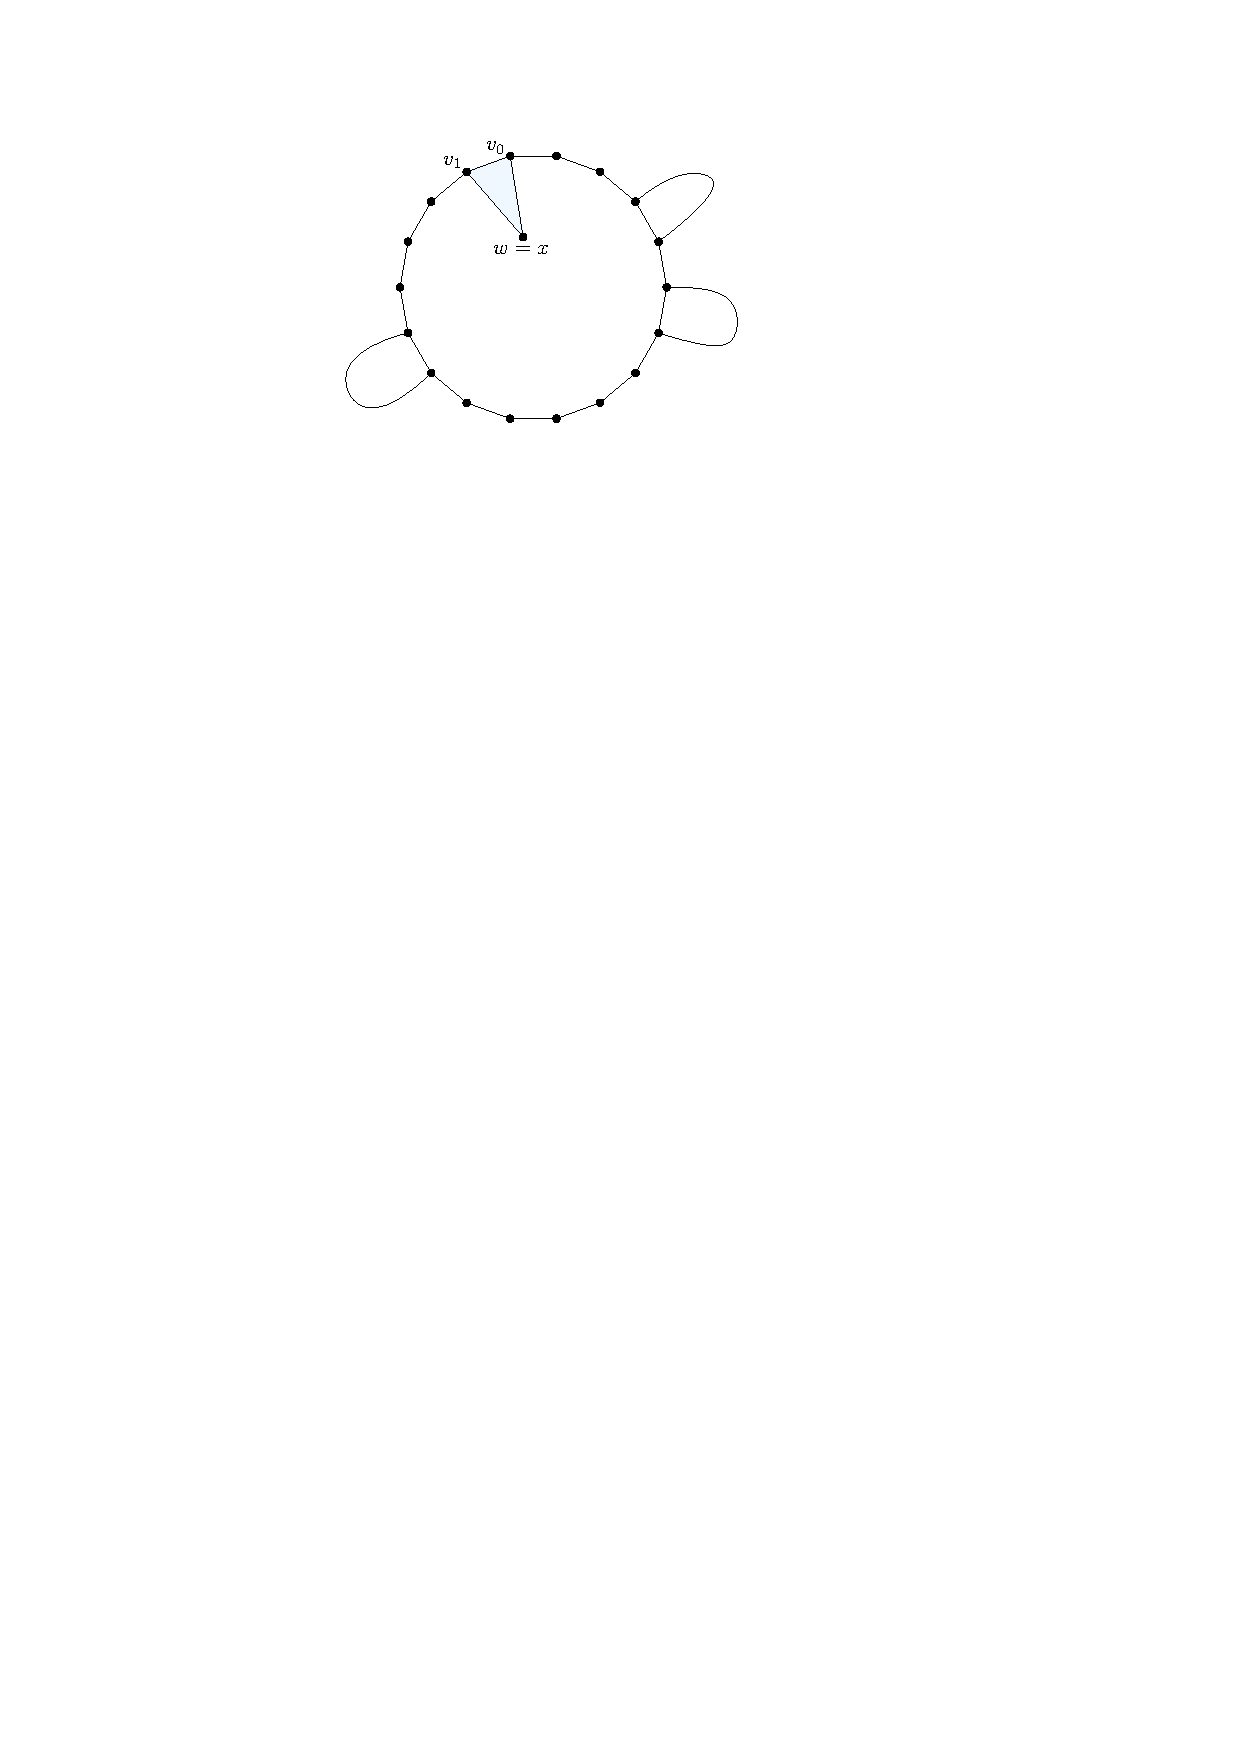
\includegraphics[page=1]{figs/degree_2_outer_neighbour} &
       \includegraphics[page=2]{figs/degree_2_outer_neighbour}
     \end{tabular}
     \caption{The proof of \cref{degree_2_outer_neighbour}.}
     \label{degree_2_outer_neighbour_fig}
   \end{figure}

   Since $w\in B(H-B(H))$, $w$ is adjacent to at least one vertex, say $v_0$, of $f$.  If $v_0v_{1}$ is a chord of $H[B(H)]$ then, by \cref{chord_incident}, $\deg^+_H(v_0)\ge 2$ and we are done, so assume that $v_0v_{1}$ is not a chord of $H[B(H)]$.  Since $H$ is dom-minimal, $H$ contains an inner face $v_0v_{1}x$ where $x$ is an inner vertex of $H$.  If $x\neq w$, then $\deg_H^+(v_0)\ge 2$ and we are done, so assume that $x=w$.  Therefore, $w$ is adjacent to $v_1$.  Thus, by assuming that $\deg^+_H(v_0)\le 2$ and that $v_0w$ is an edge of $H$ we were able to show that $v_0v_1$ is not a chord of $H[B(H)]$ and that $v_0v_1w$ is an inner face of $H$. This latter fact implies that $v_1w$ is an edge of $H$, so we can repeat this argument to establish that $\deg^+_H(v_j)\ge 2$ for some $j\in\{0,\ldots,k-1\}$ or that $v_{j}v_{j+1}$ is not a chord of $H[B(H)]$ and that $v_{j}v_{j+1}w$ is an inner face of $H$ for all $j\in\{0,\ldots,k-1\}$.  In the first case we are obviously done. In the latter case, $H$ is the graph described in the second alternative given by the lemma.
\end{proof}


Note that the next three lemmas consider the case where $H$ is a generalized near triangulation.

\begin{lem}\label{really_good}
  Let $H$ be a dom-minimal generalized near-triangulation.  Then either:
  \begin{compactenum}[(1)]
    \item $H-B(H)$ is critical; \label[p]{two_critical}
    \item $B(H)$ contains a vertex $v$ with $\deg^+_H(v)\ge 3$; or \label[p]{degree_three}
    \item $H$ contains distinct vertices $v_0$, $v_j$, and $w$ such that
    \begin{compactenum}[(a)]
      \item $v_0\in B(H)$ and $\deg^+_H(v_0)=2$;
      \item $w\in B(H-v_0)$ and $\deg^+_{H-v_0}(w)\ge 3$; and
      \item $v_j\in B(H)$ and $N^+_H(v_j) \subseteq N_H[w] $.
    \end{compactenum}
    \label[p]{two_three_pair}
  \end{compactenum}
\end{lem}

\begin{proof}
  We will assume that $H$ does not satisfy \cref{two_critical} or \cref{degree_three} and show that $H$ must satisfy \cref{two_three_pair}.  Since $H-B(H)$ is not critical, $B(H-B(H))$ contains a vertex $w$ with $\deg_{H-B(H)}(w)\ge 2$.

  Let $C$ be the biconnected component of $H$ that contains $w$, so $C$ is a near-triangulation.  Therefore, we can apply \cref{degree_2_outer_neighbour} to $C$ and $w$. Each of the first two alternatives in \cref{degree_2_outer_neighbour} are incompatible with the assumption that $\deg^+_{H-B(H)}(w)\ge 2$.  Therefore, we conclude that $N_H(w)\cap B(H)$ contains a vertex $v_0$ with $\deg^+_H(v_0)\ge 2$.  Since $H$ does not satisfy \cref{degree_three}, $\deg^+_H(v_0)< 3$, so $\deg^+_H(v_0)=2$.  Refer to \cref{really_good_fig}
  \begin{figure}
    \centering
    \begin{tabular}{ccc}
      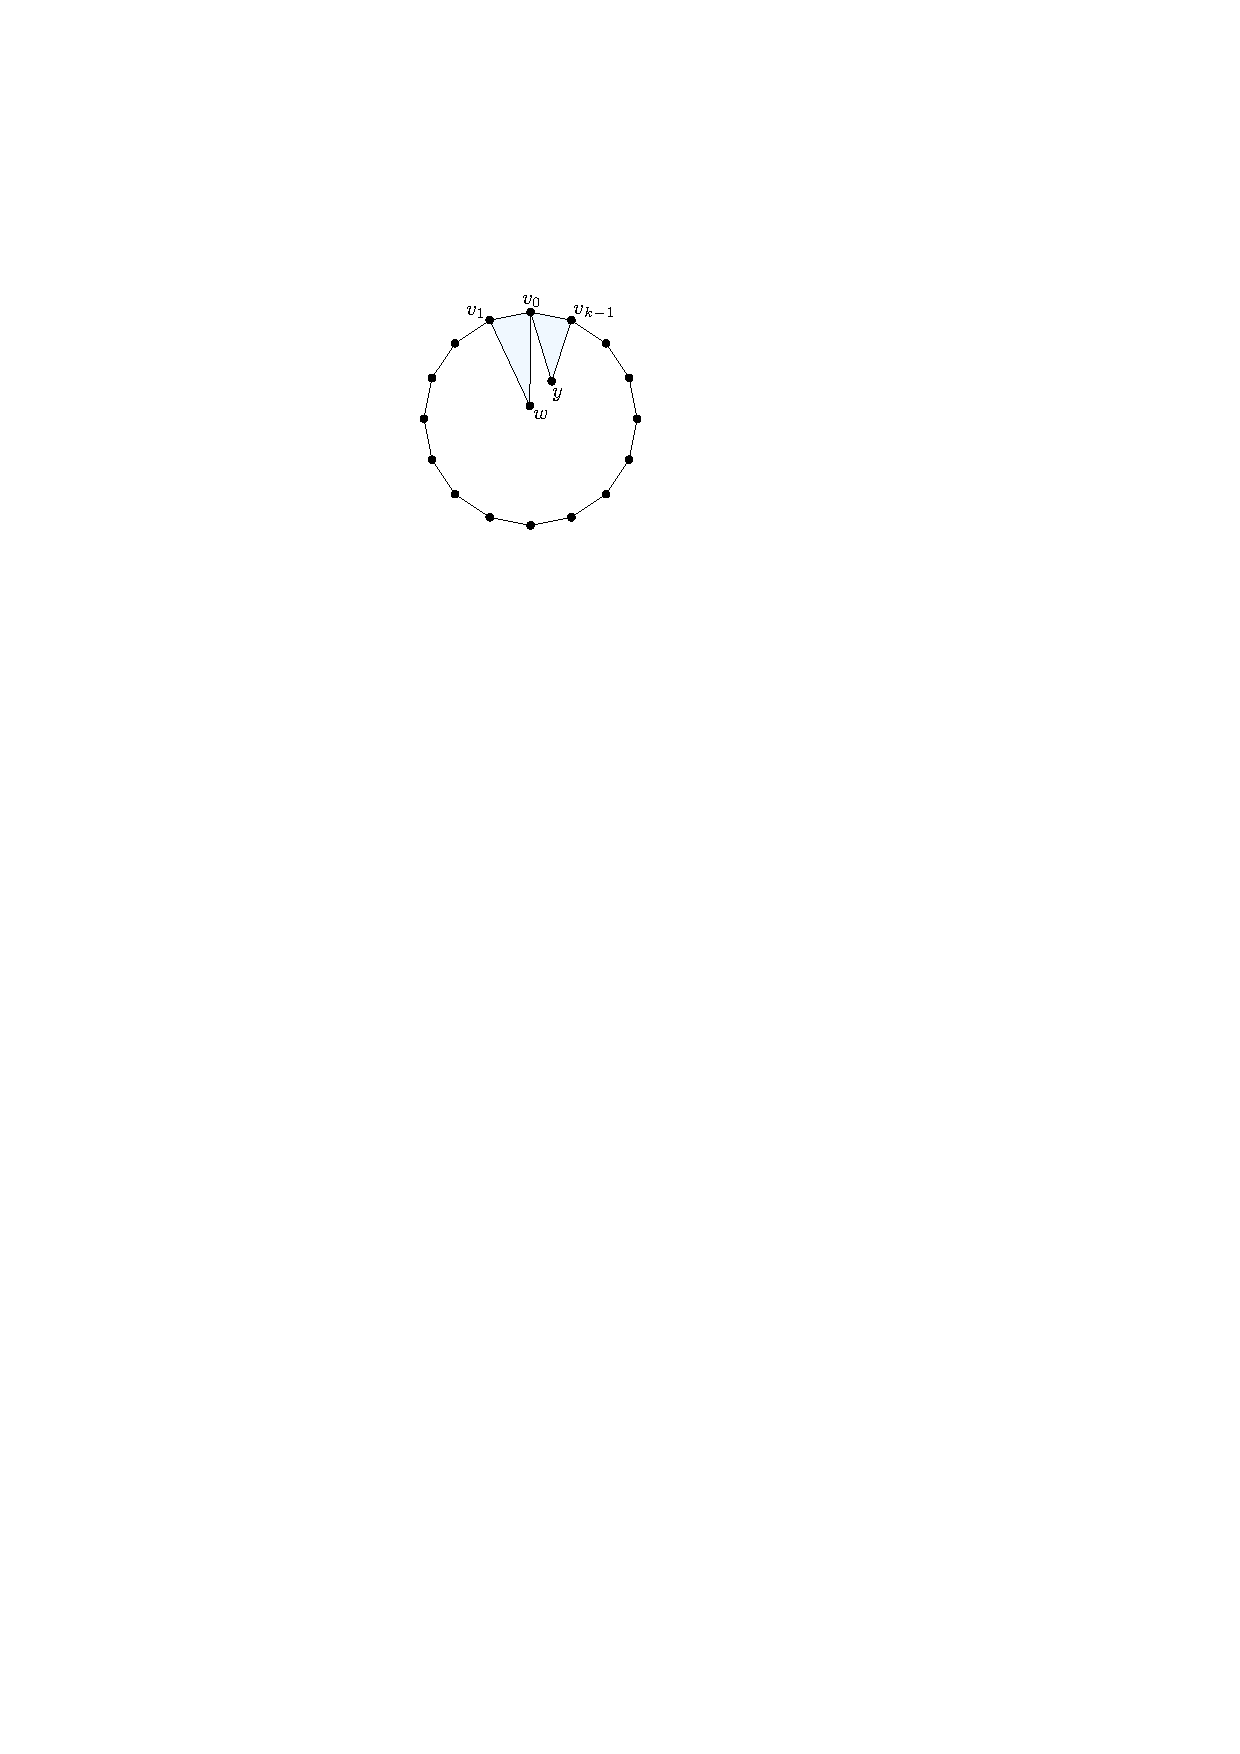
\includegraphics[page=1]{figs/really_good} &
      \includegraphics[page=2]{figs/really_good} &
      \includegraphics[page=3]{figs/really_good}
    \end{tabular}
    \caption{The proof of \cref{really_good}}
    \label{really_good_fig}
  \end{figure}

  Let $v_0,\ldots,v_{k-1}$ be the cycle that bounds the inner face $f$ of $H[B(H)]$ that contains $w$ in its interior.  Since $H$ is a near-triangulation, $H$ contains triangles $v_0v_1x$ and $v_{k-1}v_0 y$ with $x$ and $y$ in the interior of or on the boundary of $f$.  Since $f$ is a face of $H[B(H)]$ each of $x$ and $y$ is in the interior of $f$.  At least one of $x$ or $y$ is equal to $w$, say $x$, since otherwise $\deg^+_H(v_0)\ge 3$.  Therefore $v_0v_1 w$ is an inner face of $H$.  Let $j\ge 1$ be the maximum integer such that $v_{a-1}v_{a}w$ is an inner face of $H$ for all $a\in\{1,\ldots,j\}$.  Note that $j<\ell-1$ since, otherwise, the component of $H-B(H)$ that contains $w$ contains only a single vertex, contradicting the fact that $\deg^+_{H-B(H)}(w)=2$.

  Since $H$ is a near-triangulation and $f$ is a face of $H[B(H)]$, $H$ has some face $v_j v_{j+1} z$ with $z$ in the interior of $f$.  By the definition of $j$, $z\neq w$.  Therefore, $N_H^+(v_j)\supseteq \{w,z\}$ and, since $\deg^+_H(v_j)\le 2$, $N_H^+(v_j))= \{w,z\}$.  Therefore $N^+_H(v_j)\subseteq N_H[w]$.  Since $f$ is a face of $H[B(H)]$, the only neighbours of $v_j$ in $B(H)$ are $v_{j-1}$ and $v_{j+1}$. Since $H$ is a near-triangulation, this implies that $w v_j z$ is a face of $H$.  In particular $wz$ is an edge of $H$.

  All that remains is to show that $\deg^+_{H-v_0}(w)\ge 3$.  First, observe that $z$ is in $B(H-B(H))$, so $z$ does not contribute to $\deg^+_{H-B(H)}(w)$. We claim that $z$ is in $I(H-v_0)$, so $z$ does contribute to $\deg^+_{H-v_0}(w)$.   Indeed, the only other possibility is that $z$ is adjacent to $v_0$.  In this case, consider the cycle $C:=v_0,\ldots,v_j,z$.  This cycle has $w$ in its interior. The vertices of $N^+_{H-B(H)}(w)$ must be in the interior of $C$. For each $a\in\{1,\ldots,j\}$, $v_{a-1}v_a w$ is a face of $H$, so the cycle $D:=v_0,\ldots,v_j,w$ does not contain any vertices of $N^+_{H-B(H)}(w)$ in its interior.  Therefore, the vertices in $N^+_{H-B(H)}(w)$ must be in the interior of the cycle $\overline{D}:=v_0,w,z$.  Since $H$ is a near-triangulation, this implies that at least one of $v_0$ is adjacent to some vertex in $I(H)\setminus\{w,z\}$. But this is not possible since it would imply that $\deg^+_H(v_0)\ge 3$.  Therefore $v_0$ is not adjacent to $z$, so $z$ is in the interior of $H-v_0$ and $N^+_{H-v_0}(w)\supseteq N^+_{H-B(H)}(w)\uplus\{z\}$, so $\deg^+_H(w)\ge 3$.
\end{proof}


\subsection{Eliminating an Inner Leaf}

\begin{lem}\label{leaf_killer}
  Let $H$ be a dom-minimal generalized near-triangulation such that $\deg^+_H(v)\le 2$ for all $v\in B(H)$ and such that $H-B(H)$ contains a vertex $w$ with $\deg_{H-B(H)}(w)=1$.  Then there exists $v\in B(H)$ and a dom-preserving subgraph $H'$ of $H-v$ such that $|H'|\le |H|-3$ and $|B(H')|\le |B(H)|-1$.
\end{lem}

\begin{proof}
  Refer to \cref{killing_a_leaf}.
  Let $x$ be the unique neighbour of $w$ in $H-B(H)$. Since $x$ and $w$ are vertices of $H-B(X)$, $x,w\in I(H)$.  Since $w$ is an inner vertex in a near-triangulation, it is incident to $t\ge 3$ faces $v_iv_{i+1}w$ for $i\in\{0,\ldots,v_{t}\}$, with $v_0=v_t=x$.  Since $\deg_{H-B(H)}(w)=1$, $v_1,\ldots,v_{t-1}\in B(H)$.  Therefore, $H$ contains no edge $v_i v_{i+r}$ for any $i\in\{0,t-r\}$ and any $r\ge 2$.  Therefore, for each $i\in\{1,\ldots,t-1\}$, the only two inner faces of $H$ that include $v_i$ are $v_{i-1}v_iw$ and $v_iv_{i+1}w$.  Therefore $N^+_H(v_i)=\{w\}$ for each $i\in\{2,\ldots,t-2\}$ and $N^+_H(v_1)=N^+_H(v_{t-1})=\{x,w\}$.

  \begin{figure}
    \centering
    \begin{tabular}{ccc}
      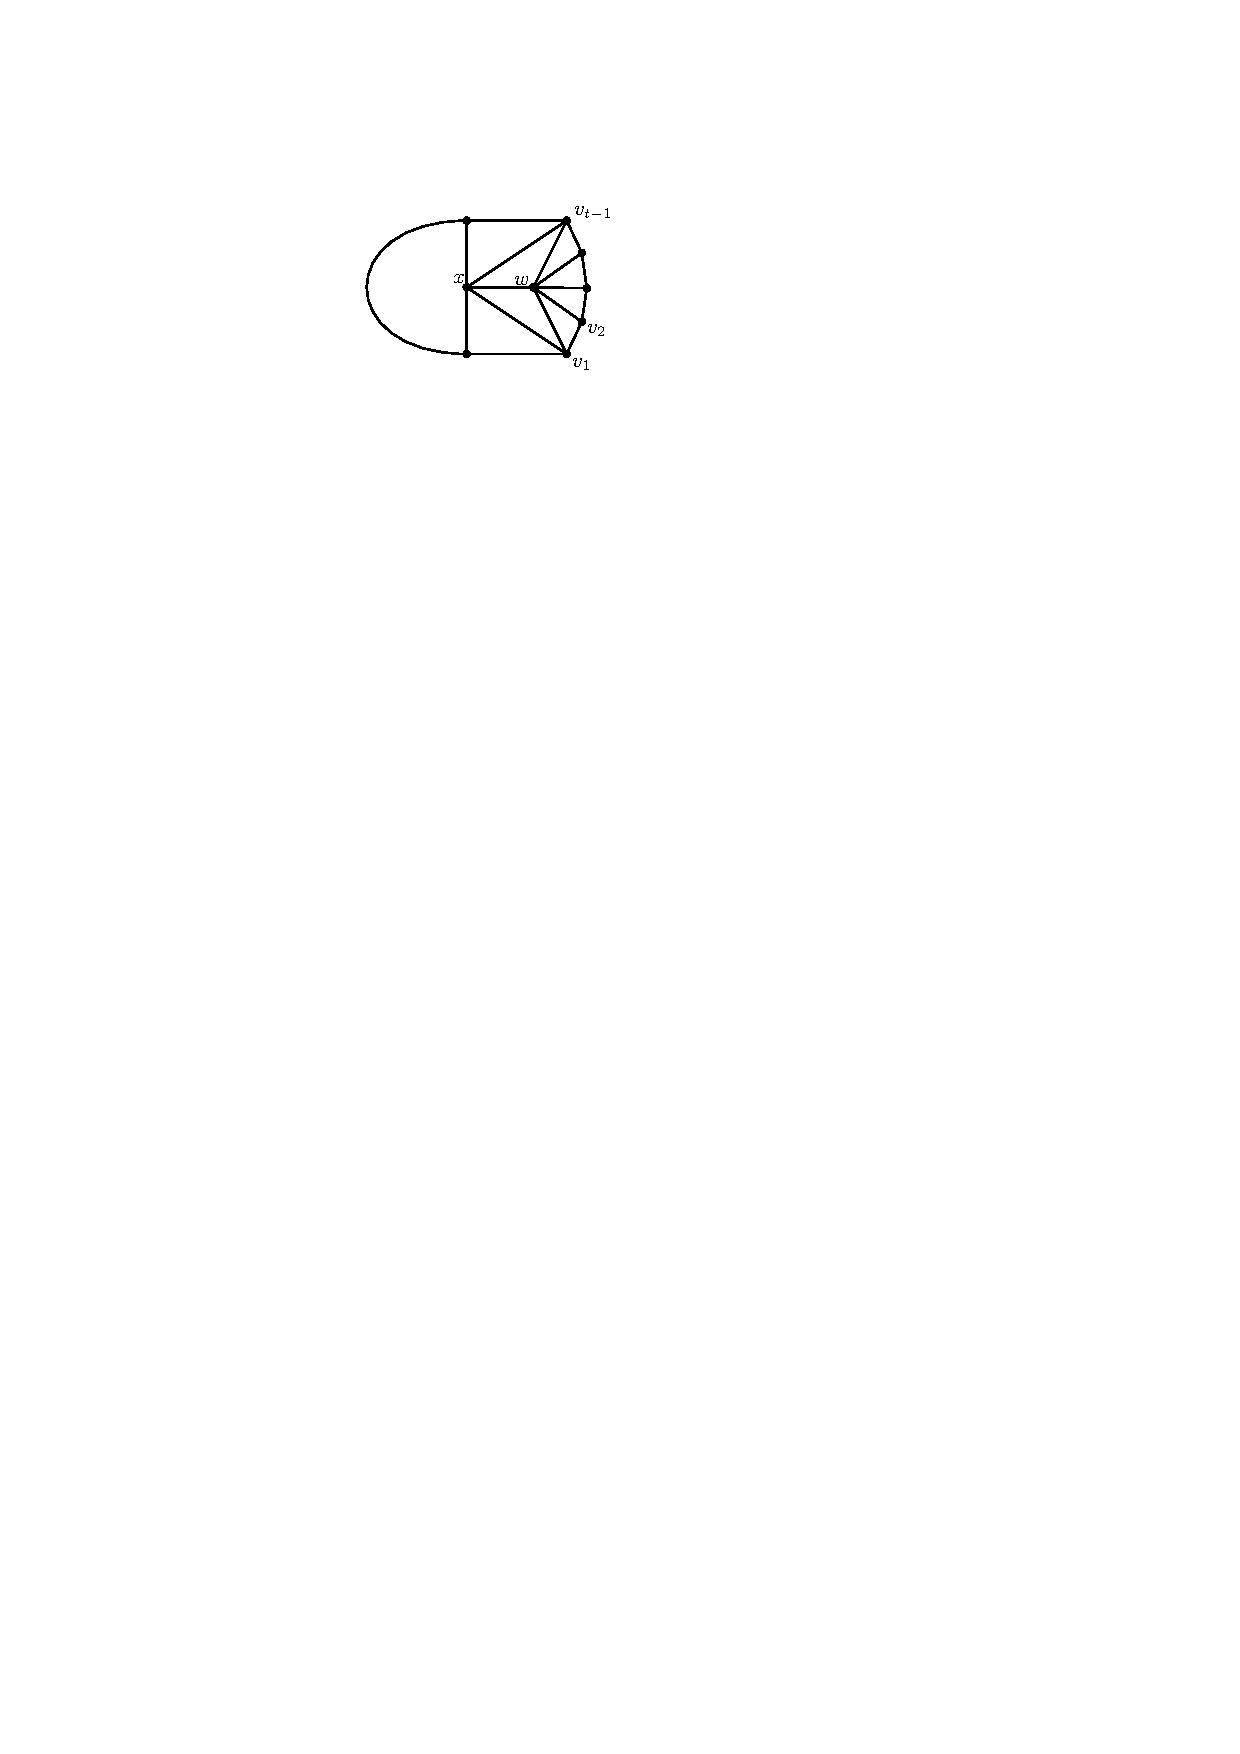
\includegraphics[page=1]{figs/killing_a_leaf} &
      \includegraphics[page=2]{figs/killing_a_leaf} &
      \includegraphics[page=3]{figs/killing_a_leaf} \\
      $H$ & $H-v$ & $H'$
    \end{tabular}
    \caption{The proof of \cref{leaf_killer}}
    \label{killing_a_leaf}
  \end{figure}

  Let $v:=v_1$ and let $H'$ be a dom-preserving subgraph of $H-v$ that is dom-minimal.  Then $w,x\in B(H-v)$.  Since $H'$ is dom-minimal, $v_1,\ldots,v_{t-1}\not\in V(H')$, by \cref{bad_vertex}.  Therefore $N_H(w)\cap V(H')=\{v_t\}=\{x\}$. Since $H'$ is dom-minimal, $w\not\in V(H')$. Therefore $V(H')\subseteq V(H)\setminus\{v_1,\ldots,v_{t-1},w\}$, so $|V(H')|\le |H|-t\le |H|-3$.  Finally, $B(H-v)=B(H)\setminus \{v\}\cup\{w,x\}$. By \cref{boundary_subset}, $B(H')\subseteq B(H-v)\setminus\{v_1,\ldots,v_{t-1},w\}\cup\{x\}$, so $|B(H')|\le |B(H)|+2-t\le |B(H)|-1$.
\end{proof}


\begin{lem}\label{degree_zero_killer}
  Let $H$ be a dom-minimal generalized near-triangulation such that $\deg^+_H(v)\le 2$ for all $v\in B(H)$ and such that $H-B(H)$ contains a vertex $w$ with $\deg_{H-B(H)}(w)=0$.  Then at least one of the following is true:
  \begin{compactenum}[(a)]
    \item there exists $v\in B(H)$ and a dom-preserving subgraph $H'$ of $H-v$ such that $|H'|\le |H|-3$ and $|B(H')|\le |B(H)|-1$; or \label[p]{kill_pair}
    \item there exists $v\in B(H)$ and a dom-preserving subgraph $H'$ of $H-v$ such that $|H'|\le |H|-4$ and $|B(H')|\le |B(H)|-3$. \label[p]{kill_k4}
  \end{compactenum}
\end{lem}

\begin{proof}
  By definition $N_H(w)\subseteq B(H)$ and, since $w$ is an inner vertex in a generalized near triangulation $|N_H(w)|\ge 3$. There are two cases to consider:
  \begin{compactenum}[(a)]
    \item There exists $v\in N_H(w)$ with $\deg^+_H(v)=2$. In this case, $N^+_H(v)=\{w,w'\}$ and the vertices $w$ and $w'$ are in a different biconnected components of $H$. \pat{Annoyingly, we have to be concerned about the possibility that the bicomponent that contains $w'$ is a more interesting one, so $\deg_{H-B(H)}(w')\ge 2$.  Still not an issue with the right definition of dom-minimal, but annoying.}

    \item $\deg^+_H(v)=1$ for all $v\in N_H(w)$.  In this case let $v$ be any vertex in $N_H(w)$ and let $H'$ be a dom-preserving subgraph of $H-v$ that is dom-minimal.  Then $w\in B(H-v)$, so $\deg^+_{H-v}(v')=0$ for all $v'\in N_H(w)$. Since $H'$ is dom-minimal, $N_H(w)\cap V(H')=\emptyset$, by \cref{bad_vertex}.  Similarly $w\not\in V(H')$, also by \cref{bad_vertex}. Therefore $|H'|\le |H-(\{w\}\cup N_H(w))| \le |H|-4$. Then $B(H-v)=B(H)\setminus\{v\}\cup\{w\}$.
    By \cref{boundary_subset}, $B(H')\subseteq B(H-v)\setminus N_H[w]$, so $|B(H')|\le |B(H)|-\deg_H(w) \le |B(H)|-3$. \qedhere
  \end{compactenum}
\end{proof}



\subsection{$2$-Critical Graphs}

\pat{Note: Change in definition}
We say that a generalized near-triangulation $H$ is \defin{$2$-critical} if $H-B(H)$ is critical, $H-B(H)$ has no vertices of degree $1$, and $\deg^+_H(v)\le 2$ for each $v\in B(H)$. (See \cref{two_critical_figure}.)
% Observe that any critical graph is also $2$-critical.
We will work our way up to a proof of the following lemma, which allows our algorithm to handle $2$-critical graphs directly, in one step:


\begin{lem}\label{two_critical_handler}
  Let $H$ be a $2$-critical generalized near-triangulation.  Then there exists $X\subseteq V(H)$ of size at most $(2|B(H-B(H))| + I(H-B(H)))/3$ that dominates $I(H)$ and such that each component of $H[X]$ contains at least one vertex in $B(H)$.
\end{lem}

\begin{figure}[htbp]
  \centering
  
\includegraphics[page=3,trim={0 15 0 0},clip]{figs/bg_layers}
  \caption{A $2$-critical generalized near-triangulation.}
  \label{two_critical_figure}
\end{figure}


%
% For any graph $H$ and two subsets $A$ and $B$ of vertices of $H$, we use $E_H(A,B):=\{vw\in E(H):v\in A, w\in B\}$ to denote the set of edges of $H$ with one endpoint in $A$ and one endpoint in $B$.


% \begin{obs}\label{degree_isolated}
%   Let $H$ be a generalized near-triangulation and let $C$ be a component of $H-B(H)$ that consists of a single vertex. Then $|E_H(V(C),B(H))|\ge 3$.
% \end{obs}
%
% \begin{proof}
%   The single vertex $w$ in $C$ is an inner vertex of the generalized near-triangulation $H$, $\deg_H(w)\ge 3$.  Since $\deg_{H-B(H)}(w)=0$, every edge incident to $w$ has an endpoint in $B(H)$, so $|E_H(V(C),B(H))|=\deg_H(w)\ge 3$.
% \end{proof}
%

% \begin{obs}\label{degree_minimum}
%   Let $H$ be a generalized near-triangulation and let $C$ be a component of $H-B(H)$. Then $|E_H(V(C),B(H))|\ge 3$.
% \end{obs}
%
% \begin{proof}
%   By contracting all the vertices of $C$ into a single vertex $w$ and eliminating multiple edges, we obtain a generalized near-triangulation $H'$ in which $w$ is an isolated vertex in $H'-B(H')=H'-B(H)$.  By \cref{degree_isolated}, $|E_{H'}(\{w\},B(H))|\ge 3$.  For every edge $wv\in E_{H'}(\{w\},B(H))$, there is at least one edge $w'v\in E_H(V(C),B(H))$, so $|E_H(V(C),B(H))|\ge |E_{H'}(\{w\},B(H))|\ge 3$.
% \end{proof}


% \begin{obs}\label{degree_minimum}
%   Let $H$ be a generalized near-triangulation and let $C$ be a component of $H-B(H)$. Then $|E_H(V(C),B(H))|\ge 3$.
% \end{obs}


\pat{Much of this section can be simplified, since we don't care about degree-$1$ vertices in $H-B(H)$ anymore.}

For a graph $H$ and a subset $A$ of the vertices of $H$, $\widehat{N}_{H}(A):=\{v\in N_H(A):|N_H(v)\cap A|\ge 2\}$. We will abuse this notation slightly by using the shorthand $\widehat{N}_H(C):=\widehat{N}_H(V(C))$ when $C$ is a subgraph of $H$. (See \cref{n2}.)
\begin{figure}[htbp]
  \centering
  \includegraphics[page=3]{figs/n2}
  \caption{An illustration of $\widehat{N}_H(A)$. Vertices of $A$ are black, vertices in $\widehat{N}_H(A)$ are orange and vertices in $N_H(A)\setminus \widehat{N}_H(A)$ are in grey.}
  \label{n2}
\end{figure}
% Let $H$ be a $2$-critical graph and let $C$ be a component of $H-B(H)$. We say that a vertex $v$ in $B(H)$ \defin{belongs} to $C$ if $|N_H(v)\cap V(C)|= 2$.  Note that, since $H$ is $2$-critical any $v\in B(H)$ belongs to at most once component of $H-B(H)$. We use the notation $S_H(C)$ to denote the set of all vertices in $B(H)$ that belong to $C$.
A \defin{corner} of a face $f$ in a plane graph $H$ is an ordered pair $(uv,vw)$ of (directed) edges in $H$ that occur consecutively around $v$ and such that the face $f$ is to the left of the path $uvw$.  Note that this includes the possibility that $u=w$, which occurs when $v$ has degree $1$. The vertex $v$ is the \defin{internal vertex} of the corner $(uv,vw)$.  For a plane graph $H$, $\corners(H)$ denotes the set of corners on the outer face of $H$.

\begin{lem}\label{corner_degree}
  Let $H$ be a $2$-critical generalized near-triangulation, and let $C$ be a component of $H-B(H)$ with at least two vertices. Then $|\widehat{N}_H(C)|\ge |\corners(C)|$.
\end{lem}

\begin{proof}
  Consider some corner $(uv, vw)$ of the outer face of $C$.  Since $u,v,w$ are in $I(H)$, $H$ contains faces $uxv$ and $vyw$ that are to the left of $uv$ and $vw$, respectively. Since the path $uvw$ is on the outer face of $C$, these faces are not faces of $H-B(H)$, so $x,y\in B(H)$.  Since $x$ is adjacent to $u$ and $v$ and $y$ is adjacent to $v$ and $w$, each of $x$ and $y$ is in $\widehat{N}_H(C)$.  We claim that $x\neq y$.  To see this, there are two cases to consider. (See \cref{uvw}.)
  \begin{figure}[htbp]
    \centering
    \begin{tabular}{cc}
      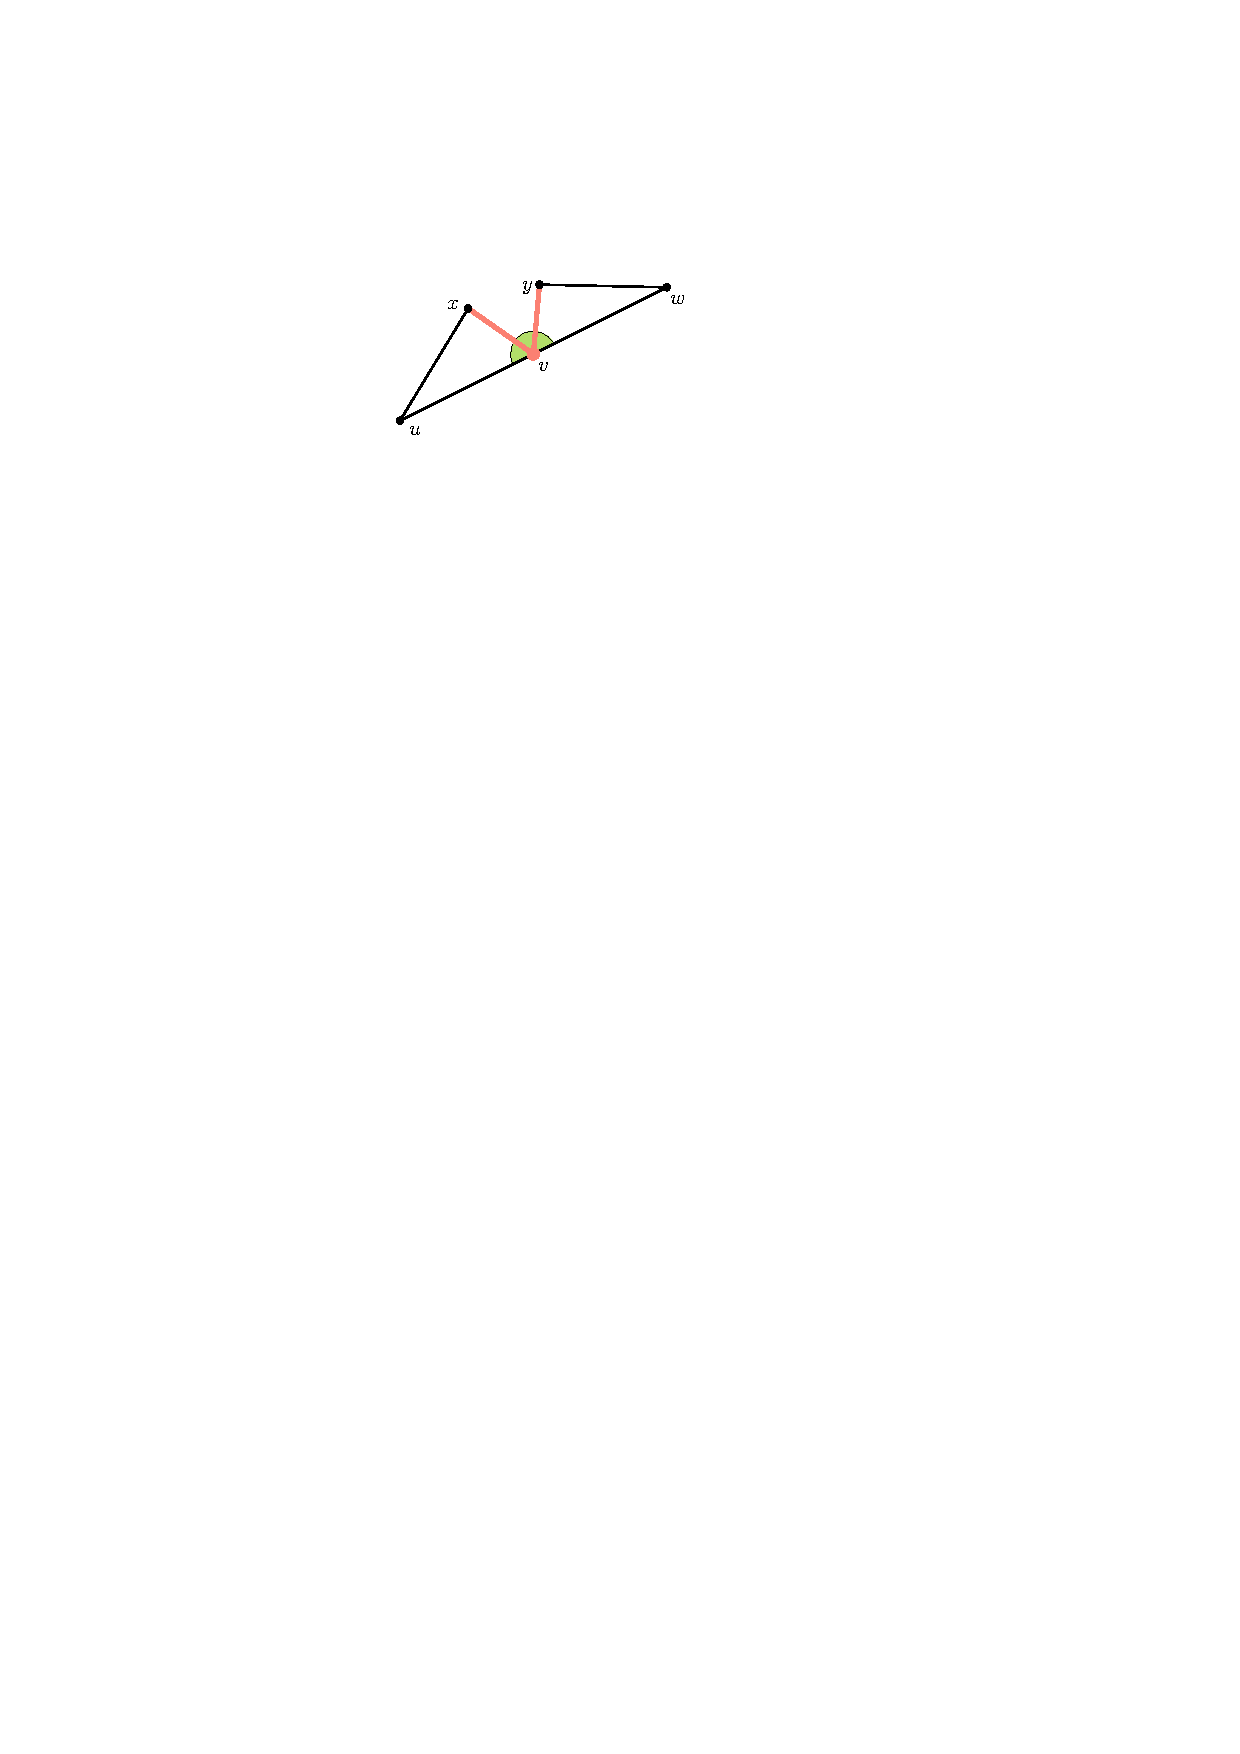
\includegraphics[page=1]{figs/corners} &
      \includegraphics[page=2]{figs/corners}
    \end{tabular}
    \caption{The two cases in the  proof of \cref{corner_degree}.}
    \label{uvw}
  \end{figure}
  \begin{compactenum}
    \item If $u\neq w$ and $x=y$ then $x\in B(H)$ is adjacent to each of $u,v,w\in I(H)$, so $\deg^+_H(x)\ge 3$, contradicting the fact that $H$ is $2$-critical.
    \item If $u=w$ and $x=y$, then there are two distinct inner faces of $H$ (one on each side of $ux$) that each have $u$, $v$, and $w$ on their boundary, which is not possible because $H$ does not have parallel edges.
  \end{compactenum}
  Therefore, the edges $vx$ and $vy$ can be assigned to the corner $(uv,vw)$. By doing this for each corner of the outer face of $C$ we obtain a mapping from the edges between $\widehat{N}_H(C)$ and $B(C)$ onto $\corners(C)$ in which each corner has two edges mapped onto it.  Therefore, the number of edges between $\widehat{N}_H(C)$ and $B(C)$ is at least $2|\corners{C}|$.  By definition, each vertex in $\widehat{N}_H(C)$ has two neighbours in $C$, so $|\widehat{N}_H(C)|\ge |\corners(C)|$.
\end{proof}

A \defin{star} is a tree with one vertex of degree at least $2$ and all other vertices of degree $1$.
For a graph $H$ and a non-negative integer $d$, let $V_d(H):=\{v\in V(H):\deg_H(v)=d\}$ be the set of vertices of $H$ having degree $d$.

\begin{lem}\label{degree_corners_and_leaves}
  Let $H$ be a $2$-critical generalized near-triangulation and let $C$ be a component of $H-B(H)$ with at least two vertices. Then $|\widehat{N}_H(C)|\ge |B(C)|$.  Furthermore, if $C$ has at least three vertices and is not a star then $|\widehat{N}_H(C)|\ge |B(C)| + |V_1(C)|$.
\end{lem}

\begin{proof}
  Each vertex in $B(C)$ is the internal vertex of at least one corner in $\corners(C)$ so, by \cref{corner_degree}, $|E_H(V(C),B(H))|\ge 2|B(C)|$.  This establishes the first part of the corollary.

  Now suppose $|C|\ge 3$ and $C$ is not a star and consider some vertex $v\in V(C)$ that is adjacent to $d\ge 1$ vertices $v_1,\ldots,v_d$ in $V_1(C)$.  Since $C$ is not a star, $v$ is also adjacent to at least one vertex $w$ in $B(C)\setminus V_1(C)$. We claim that $v$ is the internal vertex of at least $d+1$ corners in $\corners(C)$. Indeed, for each $i\in\{1,\ldots,d\}$ $v$ is the internal vertex of the corners $(x_iv,vv_i)$ and $(v_iv,vy_i)$ for some $x_i,y_i\in B(C)$.  There is at least one value of $i$ for which $x_i\not\in\{v_1,\ldots,v_d\}$.
  % and at least one value of $i$ for which $y_1\not\in\{v_1,\ldots,v_d\}$.
  For each $i\in\{1,\ldots,d\}$, there is at most one value $j$ such that $(x_iv,vv_i)=(v_jv,vy_j)$ and there is at least one value $i\in\{1,\ldots,d\}$ for which no such $j$ exists.  Therefore
  $
  |\bigcup_{i=1}^d \{(x_iv,vv_i),(v_iv,vy_i)\}| > d.
  $
  If we let $A$ denote the subset of vertices in $B(C)$ that are adjacent to at least one vertex in $V_1(C)$ we see that
  \[
    |\corners(C)| \ge |B(C)\setminus A| + |A| + |V_1(C)|
    = |B(C)| + |V_1(C)|  \enspace .
  \]
  Now the second part of the lemma follows from \cref{corner_degree}.
\end{proof}

%
% \begin{lem}\label{boundary_size}
%   Let $H$ be a $2$-critical generalized near-triangulation.  Then $|B(H)|\ge\mu(H-B(H))$.
% \end{lem}
%
% \begin{proof}
%
%   Follows immediately from \cref{degree_isolated,degree_walk} and the fact that $\deg^+_H(v)\le 2$ for all $v\in B(H)$.
% \end{proof}

For each integer $r\ge 3$, the \defin{$r$-wheel} $W_r$ is the near-triangulation whose outer face is bounded by a cycle $v_0,\ldots,v_{r-1}$ that contains a single vertex $x$ in its interior and that is adjacent to each of $v_0,\ldots,v_{r-1}$.

Note that the following lemma is about critical graphs, not $2$-critical graphs.

\begin{lem}\label{biconnected_critical}
  Let $H$ be a biconnected critical generalized near-triangulation with at least $3$ vertices and not isomorphic to $W_k$ for any even integer $k$.  Then there exists a partition $\{X_0,X_1,X_2\}$ of $V(H)$ such that
  \begin{compactenum}[(i)]
    \item For each edge $vw$ of $H[B(H)]$, $v\in X_i$ and $w\in X_j$ for some $i\neq j$;\label[p]{proper}
    \item for each $i\in\{0,1,2\}$, $X_i$ dominates $H$. \label[p]{dominates_h}
  \end{compactenum}
\end{lem}

\begin{proof}
  If $H$ is isomorphic to $W_k$ for some odd integer $k\ge 3$, then we take $X_0:=\{v_0, x\}$, $X_1:=\{v_{2i-1}:i\in\{1,\ldots,\lfloor k/2\rfloor\}$, and $X_2:=\{v_{2i}:i\in\{1,\ldots,\lfloor k/2\rfloor\}$.  It is straightforward to verify that these sets satisfy \cref{proper,dominates_h}.  (The fact that $k$ is odd ensures that $v_0$ has a neighbour $v_1\in X_1$ and $v_{k-1}\in X_2$, which ensures \cref{dominates_h}---this is not true for even $k$.)   We now assume that $H$ is not isomorphic to $W_k$ for any integer $k$.  By \cref{critical_structure}, this implies that $H$ is outerplanar or that $H[B(H)]$ has at least two inner faces.

  We now proceed by induction on $|I(H)|$.  If $|I(H)|=0$ then $H$ is an edge-maximal outerplanar graph, and therefore has a proper $3$-colouring.  We take $X_0$, $X_1$, and $X_2$ to be the three colour classes in this colouring.  This choice clearly satisfies \cref{proper}. Since each vertex of $H$ is included in at least one triangle, each vertex of $H$ is dominated by each of $X_0$, $X_1$, and $X_2$, so this choice satisfies \cref{dominates_h}.

  \begin{figure}
    \centering
    \begin{tabular}{ccc}
      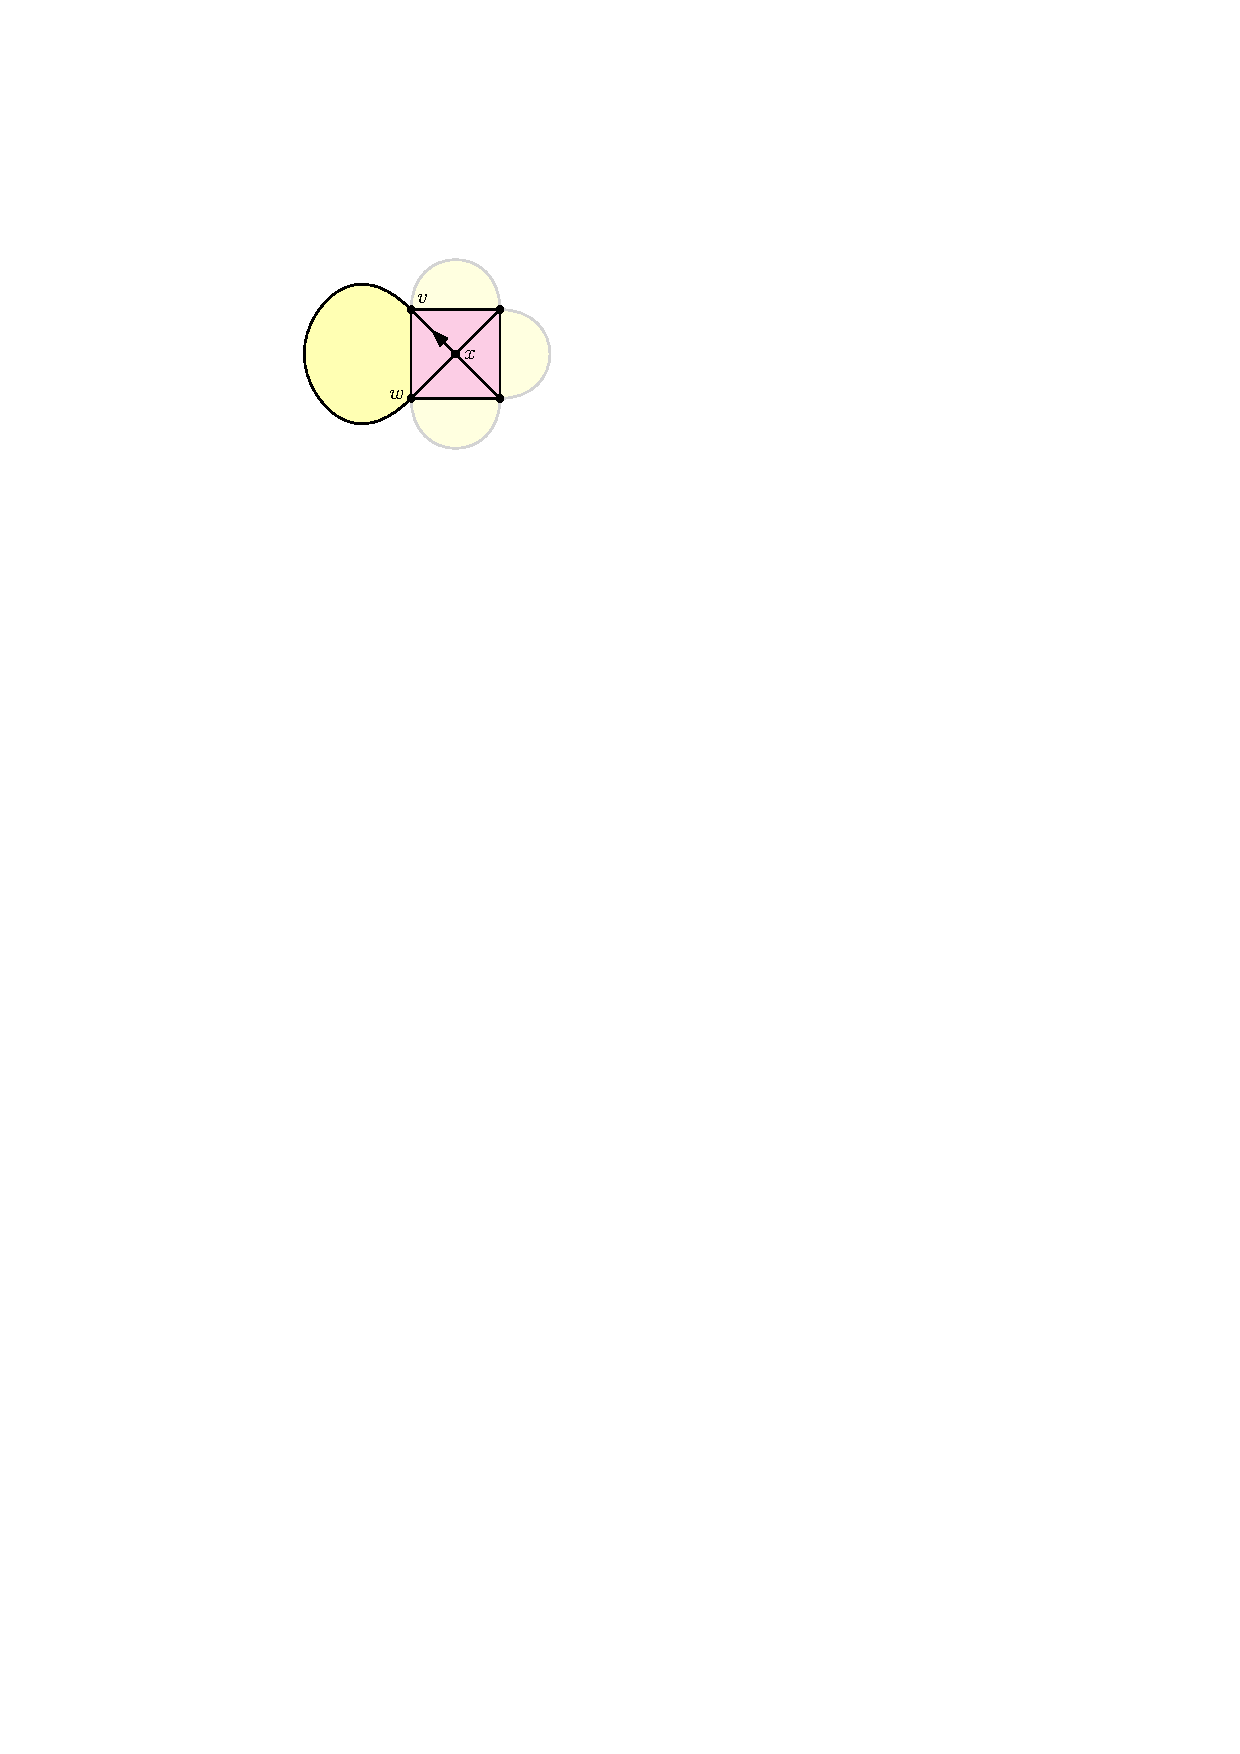
\includegraphics[page=1]{figs/biconnected} &
      \includegraphics[page=2]{figs/biconnected} &
      \includegraphics[page=3]{figs/biconnected}
    \end{tabular}
    \caption{The proof of \cref{biconnected_critical}}
    \label{contraction_proof}
  \end{figure}
  If $|I(H)|\ge 1$ then $H$ is not outerplanar.  See \cref{contraction_proof}.  Since $H$ is not isomorphic to $W_k$ for any integer $k$, $H[B(H)]$ contains at least two inner faces.  Let $x$ be an inner vertex of $H$ and let $f$ be the marked face of $H[B(H)]$ that contains $x$.
  % If $f$ has only three vertices, then we apply induction on $H':=H-x$ to obtain sets $X_0'$, $X_1'$, and $X_2'$.  We then set $X_0:=X_0'\cup\{x\}$, $X_1:=X_1'$ and $X_2:=X_2'$.  These sets satisfy \cref{proper} because every edge of $H[B(H)]$ is also an edge of $H'[B(H')]$.  These sets satisfy \cref{colourful} because $f$ is a clique of size $3$ in $H'$ so, by \cref{proper}, each $X_i$ contains at least one vertex of $f$. Now, \cref{colourful} also implies that each $X_i$ dominates $x$ and (by induction) dominates $V(H)\setminus\{x\}$, so each $X_i$ is a dominating set.
  Since $H[B(H)]$ has at least two inner faces and $H$ is biconnected, $f$ contains an edge $vw$ that is on the boundary of two faces of $H$.  Let $H'$ be the graph obtained by contracting the edge $vx$ into $v$. Then $H'[B(H')]=H[B(H)]$ and $H'$ is a biconnected critical generalized near-triangulation so we apply induction to obtain sets $X_0'$, $X_1'$ and $X_2'$.  Without loss of generality, we can assume that $v$ is in $X_1'$.  Then we set $X_0:=X_0'$, $X_1:=X_1'\cup\{x\}$ and $X_2:=X_2'$. Since $H'[B(H')]=H[B(H)]$ this clearly satisfies \cref{proper}.  Since $H'$ contains the edge $vw$ for each $w\in V(f)\setminus\{v\}$, \cref{proper} implies that the vertices of the path $f-v$ are alternately contained in $X_2$ and $X_0$.
  % In particular, since $f$ has at least three vertices these sets satisfy \cref{colourful}.

  All that remains is to show that $X_0$, $X_1$, and $X_2$ satisfy \cref{dominates_h}.  The inductive hypothesis already implies that each of these sets dominates $V(H)\setminus V(f)$.  Since $x$ is adjacent to every vertex of $f$, it is adjacent to at least one vertex of $X_0$ at least one vertex of $X_2$.  Therefore, each of $X_0$, $X_1$, and $X_2$ dominates $x$.  For each vertex $w\in V(f)\setminus\{v\}$, $w$ is adjacent to $x\in X_1$, $w\in X_{i}$ for some $i\in\{0,2\}$ and $w$ is adjacent a neighbour $w'\in X_{2-i}$ in $f$, so each of these sets dominates $w$.  Finally, since the vertex $v$ is incident to a chord of $H[B(H)]$, it is incident to a second face $f'\neq f$ of $H[B(H)]$.  Since $f$ is marked and $H$ is critical, $f'$ is not marked.  Therefore $f'$ is a triangle with one vertex in each of $X_0$, $X_1$, and $X_2$. Therefore each of these sets dominates $v$.
\end{proof}

The following lemma, illustrated in \cref{even_wheel}
 explains how we deal with even wheels:

\begin{lem}\label{wheelie}
  Let $H:=W_k$ for some even integer $k\ge 4$ and let $v$ be any vertex in $B(H)$.  Then there exists a partition $\{X_0,X_1,X_2\}$ of $V(H)$ such that
  \begin{compactenum}[(i)]
    \item For each edge $vw$ of $H[B(H)]$, $v\in X_i$ and $w\in X_j$ for some $i\neq j$;\label[p]{proper2}
    % \item For each inner face $f$ of $H[B(H)]$ and each $i\in\{0,1,2\}$, $V(f)\cap X_i\neq\emptyset$; and \label[p]{colourful}
    % that contains $x_f\in I(H)$ in its interior, exactly one vertex $v_f$ of $f$ is in the set $X_i$ that contains $x$ and $v_f$ is incident to a chord of $H[B(H)]$. \pat{Define chord.}
    \item $X_0$ dominates $V(H)\setminus\{v\}$ and $X_1$ and $X_2$ each dominate $H$. \label[p]{weak_dominates_h}
  \end{compactenum}
\end{lem}

\begin{figure}
  \centering
  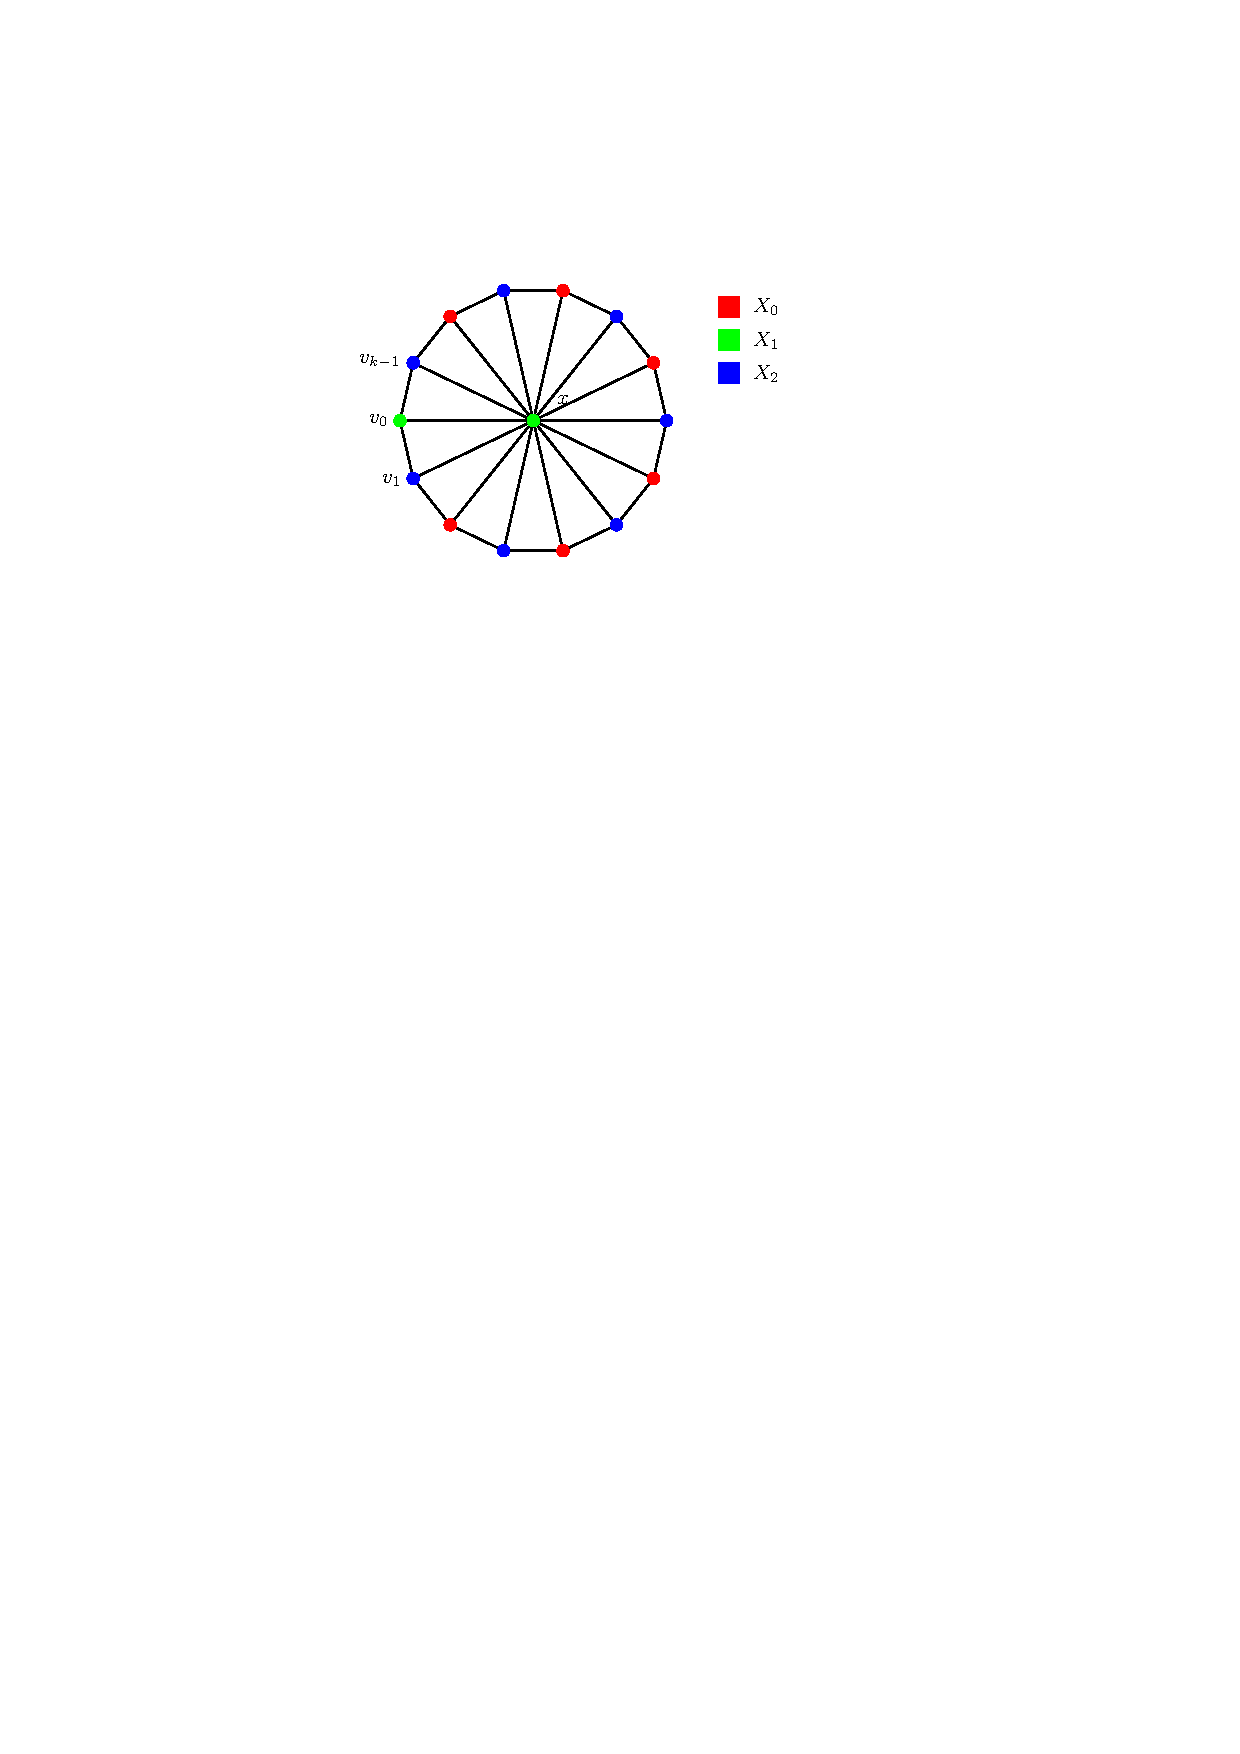
\includegraphics{figs/even_wheel}
  \caption{Partitioning the vertices of an even wheel into sets $X_0$, $X_1$, and $X_2$.}
  \label{even_wheel}
\end{figure}
\begin{proof}
  Label the vertices of $W_k$ as $v_0,\ldots,v_{k-1}$ so that $v=v_0$.  Then the sets $X_1:=\{v_0, x\}$, $X_2:=\{v_{2i-1}:i\in\{1,\ldots,k/2\}\}$, and $X_0:=\{v_{2i}:i\in\{1,\ldots, k/2-1\}\}$ satisfy the requirements of the lemma.
\end{proof}


Now we drop the requirement that $H$ is biconnected.


\begin{lem}\label{critical}
  Let $H$ be a connected critical generalized near-triangulation with at least $3$ vertices, no vertices of degree $1$ and not isomorphic to $W_k$ for any even integer $k$.  Then there exists a partition $\{X_0,X_1,X_2\}$ of $V(H)$ such that
  \begin{compactenum}[(i)]
    \item for each edge $vw$ of $H[B(H)]$, $v\in X_i$ and $w\in X_j$ for some $i\neq j$;\label[p]{proper_2}
    % \item for each marked face $f$ of $H[B(H)]$ and each $i\in\{0,1,2\}$, $V(f)\cap X_i\neq\emptyset$; and \label[p]{colourful_2}
    % that contains $x_f\in I(H)$ in its interior, exactly one vertex $v_f$ of $f$ is in the set $X_i$ that contains $x$ and $v_f$ is incident to a chord of $H[B(H)]$. \pat{Define chord.}
    \item for each $i\in\{0,1,2\}$, $X_i$ dominates $H$,  \label[p]{dominates_h_minus_l}
  \end{compactenum}
\end{lem}

\begin{proof}
  The proof is by induction on $|H|$.  First, suppose $|H|=3$. Since $H$ is connected and has no vertices of degree $1$ then $H$ is a triangle $v_0v_1v_2$. We take $X_i:=\{v_i\}$ for each $i\in\{0,1,2\}$.  Clearly these sets satisfy the requirements of the lemma.

  % If $L\neq\emptyset$ then let $z$ be a vertex in $L$ and let $z_r,\ldots,z_0$ the maximal path in $H$ such that $z=z_r$ and each of $z_1,\ldots,z_{r-1}$ has degree $2$ in $H$. Consider the graph $H':=H-\{z_1,\ldots,z_{r}\}$.
  % \begin{enumerate}
  %   \item If $z_0\in L$, then $H'$ is the graph that contains only $z_0$ and $H=z_r,\ldots,z_0$ is a path.  In this case $L:=\{z_0,z_r\}$. We take $X_i:=\{z_j:j\equiv i\pmod 3\}$ for each $i\in\{0,1,2\}$, $L_2=\{z_0\}$.  Starting with $L_0:=L_1:=\emptyset$ and $L_2:=\{z_0\}$, we then set
  %   $L_{(r-2)\bmod 3}\gets L_{(r-2)\bmod 3} \cup \{z_r\}$.  This produces sets that satisfy the requirements of the lemma, and we are done.
  %
  %   \item If $H'$ is isomorphic to $W_k$ for some even integer $k$ then we apply \cref{wheelie} with $v=z_0$ to obtain sets $X_0'$, $X_1'$, $X_2'$, $L_0'$, $L_1'$, and $L_2'$.
  %
  %   \item Otherwise, we apply the inductive hypothesis on $H'$ to obtain sets $X_0'$, $X_1'$, $X_2'$, $L_0'$, $L_1'$, and $L_2'$.
  % \end{enumerate}
  % \begin{figure}
  %   \centering
  %   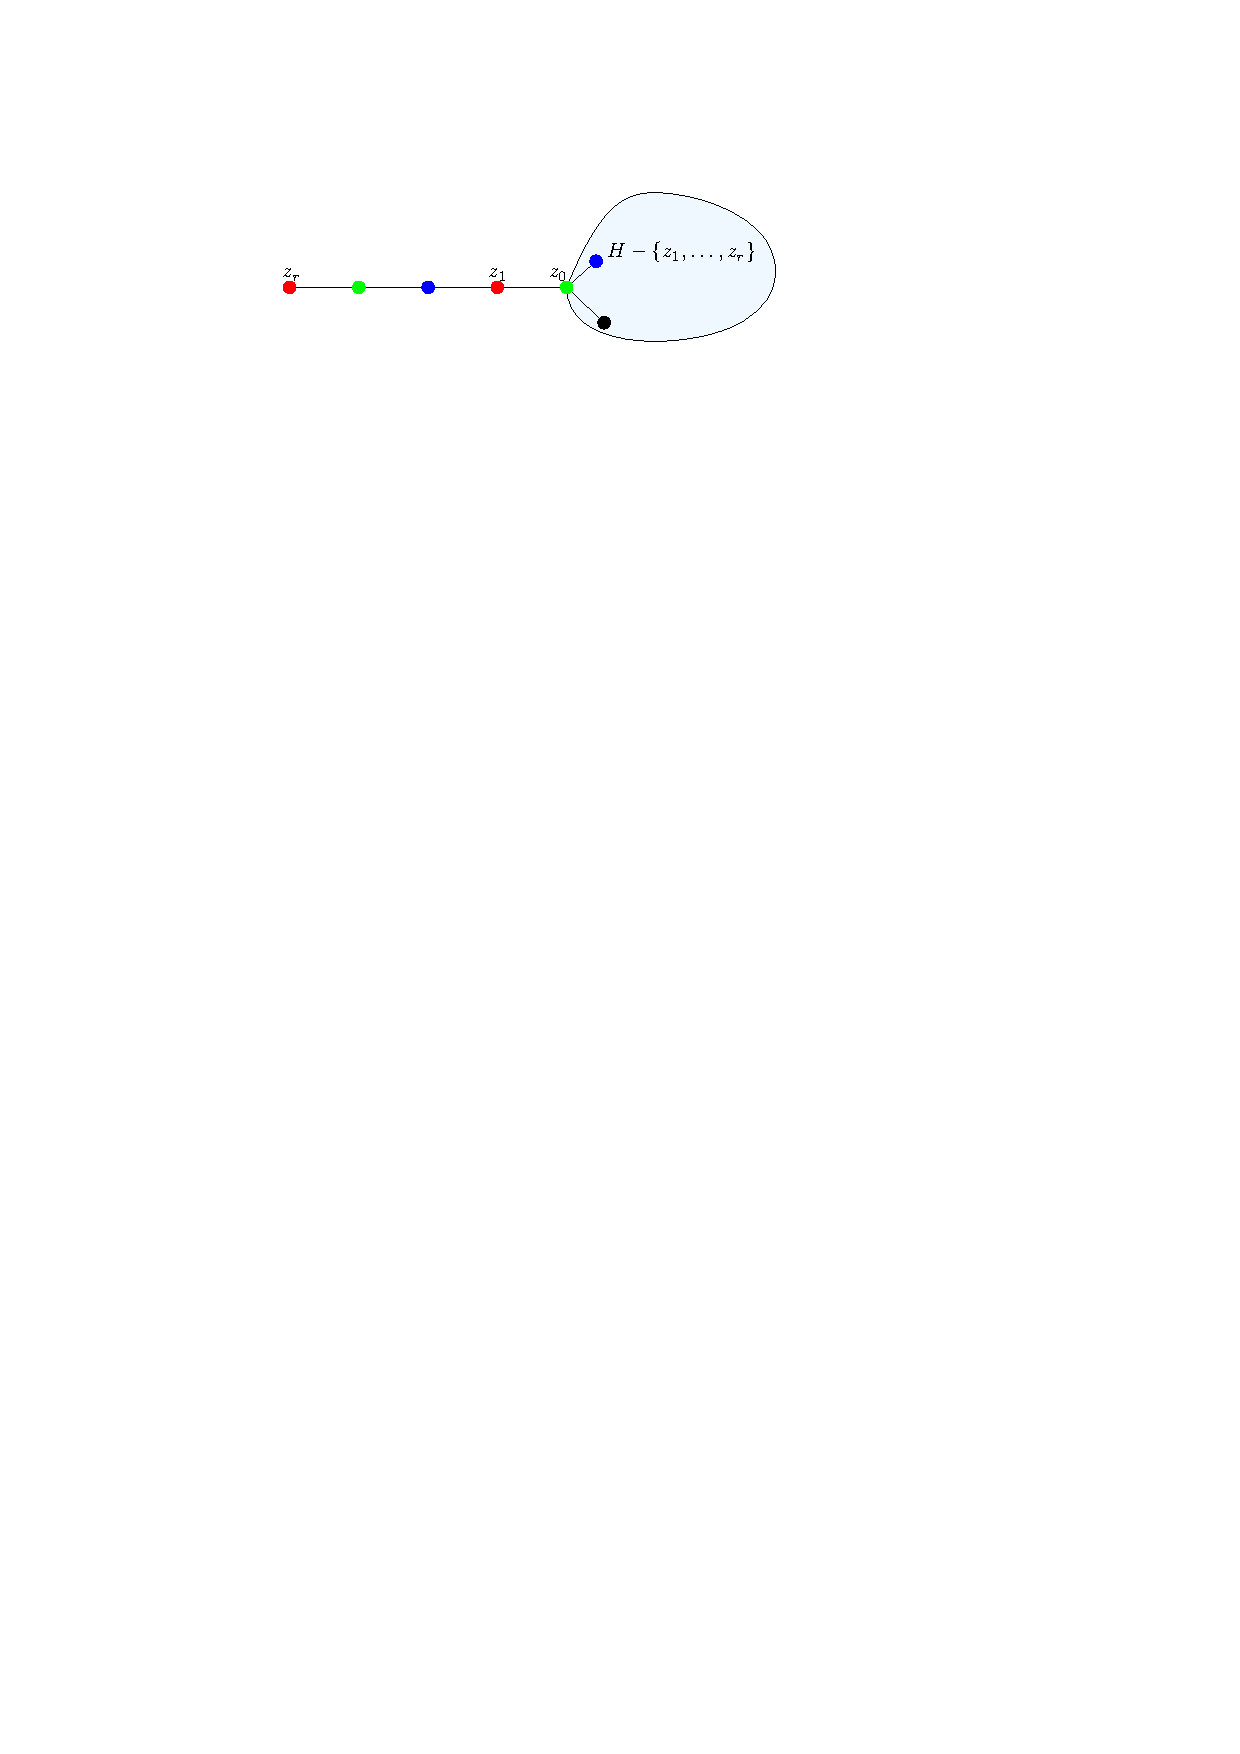
\includegraphics{figs/tail}
  %   \caption{Dealing with a degree-$1$ vertex, $z_r$, in the proof of \cref{critical}.}
  %   \label{critical_degree_one}
  % \end{figure}
  % See \cref{critical_degree_one}.
  % In the latter two cases, we may assume, without loss of generality (by renaming colours), that $z_0\in X_{1}'$.  Since $z_0\not\in L$, $\deg_H(z_0)\ge 3$ so $\deg_{H'}(z_0)\ge 2$.  Therefore we may assume, without loss of generality, that $X_1'$ and $X_2'$ each dominate $z_0$. Redefine $L_{(2-r)\bmod 3}'\gets L_{(2-r)\bmod 3}'\cup\{z_r\}$ so that $L_0'$, $L_1'$ and $L_2'$ is a partitition of $L$.  Then we take $X_i:=X_{i}'\cup\{z_j:1-j\equiv i\pmod 3\}$, $L_0:=L_0'$, $L_1:= L_1'$, and $L_2:=L_2'$.  These sets satisfy the requirements of the lemma.  Indeed, the only concern would be that $z_0$ is not dominated by $X_0$ because $z_0$ is not necessarily dominated by $X_0'$, but this does not occur because $X_0$ includes $z_1$.

  % Finally, we arrive at the case in which $L=\emptyset$.
  If $H$ is biconnected then, since $H$ is not an even wheel, we can immediately apply \cref{biconnected_critical} and we are done.  Otherwise, $H$ contains a cut vertex $v$ that separates $H$ into components $C_1,\ldots,C_k$ and such that $H':=H[V(C_1)\cup\{v\}]$ is biconnected. Since $L=\emptyset$, $H'$ has at least three vertices. If $H'$ is isomorphic to $W_k$ for some even integer $k$ then we apply \cref{wheelie} to $H'$ and $v$ to obtain sets $X_0'$, $X_1'$, and $X_2'$. Otherwise, we apply \cref{biconnected_critical} to $H'$ to obtain sets $X_0'$, $X_1'$, and $X_2'$.  In either case we may assume, without loss of generality that $v\in X_1'$, that $X_1'$ and $X_2'$ each dominate $H'$ and that $X_0'$ dominates $V(H')\setminus\{v\}$.

  Let $H'':=H-V(C_1)$. If $H''$ is isomorphic to $W_k$ for some even integer $k$ then we apply \cref{wheelie} to $H''$ and $v$ to obtain sets $X_0''$, $X_1''$, $X_2''$. Otherwise, we apply the inductive hypothesis to $H''$ to obtain sets $X_0''$, $X_1''$, $X_2''$ that each dominate $H''$. In either case we may assume, without loss of generality (by renaming) that $v\in X_1''$, that $X_1''$ and $X_2''$ each dominate $H'$ and that $X_0''$ dominates $V(H'')\setminus\{v\}$.  Then the sets $X_0:=X_0'\cup X_2''$, $X_1:=X_1'\cup X_1''$ and $X_2:=X_2'\cup X_0''$ satisfy the requirements of the lemma.  (The only concern is whether each set dominates $v$, but this is guaranteed by the fact that $v\in X_1$, and that $X_2'\subseteq X_2$ and $X_2''\subseteq X_0$ each dominate $v$.)
\end{proof}


\begin{lem}\label{three_sets_coverage}
  Let $H$ be a $2$-critical generalized near-triangulation.  Then there exists $X_0,X_1,X_2\subseteq V(H)$ such that
  \begin{compactenum}[(i)]
    \item $|X_0|+|X_1|+|X_2| \le 2|B(H-B(H))|+|I(H-B(H))|$; \label[p]{total_size}
    \item for each $i\in\{0,1,2\}$, $X_i$ dominates $I(H)$ in $H$; and \label[p]{dominates_i}
    \item for each $i\in\{0,1,2\}$, each component of $H[X_i]$ contains at least one vertex in $B(H)$. \label[p]{connectivity}
  \end{compactenum}
\end{lem}

\begin{proof}
  Refer to \cref{covers}.
  Let $H_1:=H-B(H)$, let $\mathcal{C}$ be the set of components of $H_1$, let $\mathcal{C}_1$ be the set of components of $H_1$ having exactly one vertex,
  % let $\mathcal{C}_2$ be the set of components of $H_1$ having exactly two vertices, let $\mathcal{C}_\star$ be the set of components of $H_1$ that are stars,
  and let $\mathcal{C}_{\boxtimes}$ be the set of components of $H_1$ that are even wheels.
  % , and let $\overline{\mathcal{C}}:=\mathcal{C}$ be the set of componets of $H_1$ that are not in $\mathcal{C}_1\cup \mathcal{C}_{\boxplus}$.

  \begin{figure}
    \centering
    
\includegraphics[page=5,trim={0 10 0 0},clip]{figs/bg_layers}
    \caption{Partitioning the components of $H-B(H)$ into the classes $\mathcal{C}_1$, $\mathcal{C}_2$, $\mathcal{C}_{\star}$, and $\overline{\mathcal{C}}$.  Edges within each component are ultrafat. Each class is drawn so that it contains the associated vertices of $B(H)$.}
    \label{covers}
  \end{figure}

  % By \cref{boundary_vs_leaves}, to satisfy \cref{boundary_size} it suffices to construct three sets whose total size is not more than $|I_1|+\mu(H_1)=|I_1|+2|Z| + |L| + |B_1|$.

  % For each component $C$ in $\mathcal{C}_2$ we choose one vertex $v$ in $B(H)$ that dominates $V(C)$ and place $v$ in each of $X_0$, $X_1$, and $X_2$. This contributes a total of $3|\mathcal{C}_2|$ vertices in $X_0$, $X_1$, and $X_2$. On the other hand, $\sum_{C\in \mathcal{C}_2} |C|=2|\mathcal{C}_2|$ and, by \cref{degree_corners_and_leaves},  $\sum_{C\in \mathcal{C}_2} |\widehat{N}_H(C)|\ge 2|\mathcal{C}_2|$.

  % For each component $C$ in $\mathcal{C}_{\star}$ we choose the vertex $w\in C$ that dominates the star $C$ and a vertex $v\in B(H)$ adjacent to $w$.  We place $\{v,w\}$ in each of $X_0$, $X_1$, and $X_2$.  This contributes a total of $6|\mathcal{C}_{\star}|$ vertices to $X_0$, $X_1$, and $X_2$.  On the other hand, $\sum_{C\in \mathcal{C}_{\star}} |C|\ge 3|\mathcal{C}_{\star}|$ and, by \cref{degree_corners_and_leaves}, $\sum_{C\in \mathcal{C}_{\star}} |\widehat{N}_H(C)|\ge 3|\mathcal{C}_\star|$. \pat{Remark: this inequality is always loose, in fact $|\widehat{N}_H(C)|\ge 4|C|$}

  % For each component $C$ in $\mathcal{C}_{1}$ we choose an arbitrary vertex $v$ in $B(C)$ and add it to each of $X_1$, $X_2$, and $X_3$.  This contributes at most $|\mathcal{C}_1|$ to the total size of these sets.  On the other hand, for each $v
  %
  %
  % the vertex $x$

  For each component $C$ in $\mathcal{C}_{\boxtimes}$ we choose the vertex $x$ that dominates $C$, some vertex $w$ in $B(C)$ and some vertex $v\in B(H)$ adjacent to $w$.  We add $\{v,w,x\}$ to each of $X_0$, $X_1$, and $X_2$.  This contributes a total of $9|\mathcal{C}_{\boxplus}|$ vertices to $X_0$, $X_1$, and $X_2$. On the other hand, $|B(C)|\ge 4$ and $|I(C)|\ge 1$ for each $C\in \mathcal{C}_{\boxplus}$, so
  $\sum_{C\in \mathcal{C}_{\boxplus}} (2|B(C)| + I(C))\ge (2\cdot 4+1)|\mathcal{C}_{\boxplus}| = 9|\mathcal{C}_{\boxplus}|$.

  For each component $C$ in $\mathcal{C}\setminus(\mathcal{C}_{\boxplus}\cup\mathcal{C}_1)$, we apply \cref{biconnected_critical} to obtain sets $X_0'$, $X_1'$, $X_2'$.
  For each $j\in\{0,1,2\}$ we add $X_j'$ to $X_j$.  The total number of vertices added to $X_0$, $X_1$, and $X_2$ by this step is $\sum_{C\in\mathcal{C}\setminus(\mathcal{C}_{\boxplus}\cup\mathcal{C}_1)}(|C|+|B(C)|)=\sum_{C\in\mathcal{C}\setminus(\mathcal{C}_{\boxplus}\cup\mathcal{C}_1)}(2|B(C)|+|I(C)|)$.

   % and, by \cref{degree_corners_and_leaves}, $\sum_{C\in \mathcal{C}_{\star}} |\widehat{N}_H(C)|\ge 4|\mathcal{C}_{\boxtimes}|$.

  % On the other hand, by \cref{degree_corners_and_leaves}, $\sum_{C\in \overline{\mathcal{C}}} |\widehat{N}_H(C)|\ge \sum_{C\in \overline{\mathcal{C}}} (|B(C)|+|V_1(C)|)$.

  Finally, it remains to consider the components of $H_1$ that are in $\mathcal{C}_1$. Each of these components is a single vertex in $V_0(H_1)$. These we deal with as a group. For each $w\in V_0(H_1)$, let $H_w:=H[N_H[w]]$ and let $Q:=\bigcup_{w\in V_0(H_1)} H_w$.  For each $w\in V_0(V_1)$, the graph $H_w$ is isomorphic to $W_k$ for some $k\ge 3$, $B(H_w)\subseteq B(H)$ and, for any component $C$ of $H_1$ other than the one containing $w$, $\widehat{N}_H(C)\cap B(H_w)=\emptyset$. In other words, none of the vertices in $B(Q)$ has been counted in the preceding paragraphs.  We construct a $X'\subseteq B(Q)\subseteq B(H)$ that dominates $I(Q)=V_0(V_1)$ by repeating the following as long as there is vertex $w$ in $V_0(H_1)$ not dominated by $X'$:
  \begin{compactenum}
    \item  If $H_w$ has no vertex in common with $H_{w'}$ for any $w'\in V_0(H_1)\setminus\{w\}$ then we add any vertex of $B(H_w)$ to $X'$.
    \item Otherwise there exists $w'\neq w$ and $v\in B(H_w)\cap B(H_{w'})$ and we add $v$ to $X'$.
  \end{compactenum}
  In the first case, the four vertices of $B(H_w)$ are no longer relevant and can be removed from $Q$, so $2|V(Q)\cap B(H_1)| + |V(Q)|\cap I(H_1)$ decreases by $7$. In the second case, the vertices $v$, $w$, and $w'$ are no longer relevant and can be removed from $Q$, so $2|V(Q)\cap B(H_1)| + |V(Q)|\cap I(H_1)$ decreases by $4$. Thus, at each step we add one vertex to $X'$ and $2|V(Q)\cap B(H_1)| + |V(Q)|\cap I(H_1)$ decreases by at least $4$, so |X'|\le (2|B(Q)|+I(Q))/4$. We finish by adding $X'$ to each of $X_1$, $X_2$, and $X_3$, which only increases their total size by at most $3|X'| <  2|B(Q)|+I(Q)$.


  Putting everything together we get that
  \[
   |X_1|+|X_2|+|X_3| \le \sum_{C\in\mathcal{C}} (|C|+\widehat{N}_H(C)) + |Q|
   \le \sum_{C\in\mathcal{C}} |C| + B(H) = I(H)+B(H)=|H| \enspace . \qedhere
  \]
\end{proof}

\begin{proof}[Proof of \cref{two_critical_handler}]
  Take $X$ to be the smallest of the three sets $X_0$, $X_1$, and $X_2$ guaranteed by \cref{three_sets_coverage}.
\end{proof}


\subsection{The Algorithm}

All of this has been leading up to a variant  $\textsc{SimpleGreedy}(G)$ that we call $\textsc{BetterGreedy}(G)$.  Suppose we have already chosen $\Delta_0,\ldots,\Delta_{i-1}$ for some $i\ge 0$ and we now want to choose $\Delta_i$.  Let $X_i:=\bigcup_{j=0}^{i-1}\Delta_j$, let $G_i$ be a dom-preserving subgraph of $G-X_i$ that is dom-minimal, and let $v_i$ be a vertex in $B(G_i)$ that maximizes $\deg^+_{G_i}(v_i)$.  During iteration $i\ge 0$, there are now three cases to consider:
\begin{compactenum}[{[}bg1{]}]
    \item If $\deg^+_{G_i}(v_i)\ge 3$ then we set $\Delta_i\gets\{v_i\}$.
    \label[bg]{bg_high_degree}
    \item If there exists distinct $u,v\in B(G_i)$ and $w\in B(G_i-B(G_i))$ such that $\deg^+_{G_i}(v)=2$, $\deg^+_{G_i-v}(w)\ge 3$, and $N^+_{G_i}(u)\subseteq N_{G_i}(w)$ then set $\Delta_i:=\{v,w\}$.
    \label[bg]{bg_two_three}
    \item Otherwise, $G_i$ is $2$-critical and $i+1=r$.  By \cref{two_critical_handler}, there exists $\Delta_{r-1}\subseteq V(G_i)$ of size at most $|B(G_i-B(G_i))|/3 + |I(G_i[I(G_i)])|$ that dominates $I(G_i)$.
    \label[bg]{bg_two_critical}
\end{compactenum}

\begin{figure}
  \centering
  
\includegraphics[page=2,trim={0 28 0 23},clip]{figs/bg_layers.pdf} \\[0ex]
  $G[R\cup S]$ \\[2ex]
  
\includegraphics[page=3,trim={0 18 0 10},clip]{figs/bg_layers.pdf} \\
  $G[Q\cup R\cup S]$ \\[2ex]
  
\includegraphics[page=4]{figs/bg_layers.pdf} \\
  $G[X\cup Q\cup R\cup S]$ \\[2ex]
  \caption{A useful figure?}
\end{figure}
\begin{thm}\label{best_greedy}
  When applied to an $n$-vertex triangulation $G$,  $\textsc{BetterGreedy}(G)$ produces a connected dominating set $X_r$ of size at most $10n/21\pm O(1)$.
\end{thm}
% \hussein{Is adding the following inequality to the constrains helpful  $r \leq |E|/4 \leq 3n/4 - 3/2$? I don t think so  } \pat{No: The optimal is achieve when $r\approx n/7$}
\begin{proof}
  For each integer $t\ge 3$, let $x_t$ be the number of times $\textsc{BetterGreedy}(G)$ falls into case \cref{bg_high_degree} and chooses $v_i$ such that $\deg^+_{G_i}(v_i)=t$ and let $z$ be the number of times $\textsc{BetterGreedy}(G)$ falls into case \cref{bg_two_three}.  Then
  \[
     D:=\left|N_G[X_{r-1}]\right| = 3 + \sum_{t\ge 3}tx_t + 5z \enspace .
  \]
  is the size of the set dominated $X_{r-1}$ immediately before the final iteration of $\textsc{BetterGreedy}(G)$.

  Let $Q:=|B(G_{r-1})|$, let $R:=|B(G_{r-1}-B(G_{r-1}))|$, and let $S:=|I(G_{r-1}-B(G_{r-1}))$.  In words: $Q$ is the size of the boundary of the $2$-critical graph $G_{r-1}$; $R$ is the size of the of the boundary of the critical graph obtained after removing the boundary of $G_{r-1}$; and $S$ is the independent set of vertices in the interior of this critical graph.
  Then, by \cref{degree_corners_and_leaves} and \cref{base_case}

  \begin{equation}
    Q \ge R \ge 3S \enspace . \label{best2}
  \end{equation}
  By definition $r-1 = \sum_{t\ge 3}x_t+z$.
  As in the proofs of \cref{simple_greedy}, $D+|I(G_i)|=D+R+S=n$, so we get the constraint:
  \begin{equation}
    n = D+R+S = \sum_{t\ge 3} tx_t + 5z + R + S \label{best3} \enspace .
  \end{equation}
  Since $B(G_{r-1})\subseteq N_G(X_{r-1})$, $D \ge |X_{r-1}|+|B(G_{r-1})|=r-1+Q$, so
  \begin{equation}
    n = D+R+S \ge r-1 + Q + R + S \enspace . \label{best4}
  \end{equation}
  Finally, the size $Q$ of the boundary $B(G_{r-1})$ is at most
  \begin{equation}
    Q \le 3 + \sum_{t\ge 3}(t-1)x_t + 2z \enspace . \label{best5}
  \end{equation}
  By \cref{two_critical_handler}, the size of $\Delta_{r-1}$ is at most $2(R+S)/3$, so the total size of the final set $X$ is at most
  \begin{equation}
    r-1 + z + (Q+R+S)2(R + S)/3 \enspace .  \label{best_objective}
  \end{equation}
  We can eliminate the variables $x_t$ for $t\ge 4$:
  \begin{clm}
    In any assignment of non-negative values to $Q, R, S$, $z$, and $x_3,x_4\ldots$ that maximizes \cref{best_objective} subject to \cref{best2,best3,best4,best5}, $x_t=0$ for all $t\ge 4$.
  \end{clm}
  \begin{clmproof}
     If $x_t = c >0$ for some $t\ge 3$, then we can set $x_t\gets 0$, $z\gets z+tc/?$, \ldots \pat{Finish this....}
  \end{clmproof}
  \begin{clm}
    In any assignment of non-negative values to $Q, R, S$, $z$, and $x_3,x_4\ldots$ that maximizes \cref{best_objective} subject to \cref{best2,best3,best4,best5}, $z=0$.
  \end{clm}
  \begin{clmproof}
    If $z = c >0$  then we can set $z\gets 0$, $x_3\gets x_3+5c/3$, $Q\gets Q+10c/3-2c=Q+4c/3$, $R\gets 10c/3-2c=Q+4c/3$, and $S\gets 10c/9-2c/3=S+4c/9$. Then the objective function \cref{best_objective} increases by $(5/3+4/3+4/9)c >0$.  \Cref{best2} is still satisfied because the quantities $Q$, $R$, and $3S$ change by exactly the same amount.  \Cref{best3} is still satisfied because the right hand side decreases by $(5-4/3+4/3)c=7c/3$. \Cref{best4} still holds because the right hand side decreases by $4c/3 + 4c/3 +4c/9 - 5c/3>0$  \Cref{best5} still holds because the left hand side decreases by $4c/3$ and the right hand side increases by $10c/3 - 2c=4c/3$.

  \end{clmproof}
  Therefore, \cref{best2,best3,best4,best5} are inequalities in four non-negative variables $x_3$, $Q$, $R$ and $S$.  Maximizing \cref{best_objective} subject to these constraints is an easy linear programming exercise and the maximum is achieved when \pat{Correct these: $x_3=(n-6)/5$, $Q=R=(2n+3)/5$, $S=0$, giving a final bound of $|X|\le r-1+R/3\le (7n-12)/15$---See Sage Code in the appendix.}.
\end{proof}


%%%%%%%% The application section %%%%

\section{An Application to Graph Drawing}
\label{one_bend}
This section illustrates an application for a connected dominating set in planar triangulation. We show that every connected dominating set induces a $1$-bend collinear set. An \defin{$h$-bend drawing} of a planar graph $G$ is an embedding in the plane such that every edge is drawn as a sequence of at most $h + 1$ straight line segment. For $h \in \mathbb{N}$, a set $S \subseteq V(G)$ is \defin{$h$-bend collinear set} if there is an $h$-bend drawing of $G$ that maps $S$ to a straight line.

We are interested in finding bounds on the size of $h$-bend collinear set. For $0$-bend collinear set, constructions of non-Hamiltonian cubic triconnected planar graphs \cite{DBLP:journals/jct/GrunbaumW73,DBLP:conf/wg/RavskyV11,DBLP:journals/jocg/LozzoDFMR18} imply that planar triangulation has a 0-bend collinear set of size at most $O(n^{\sigma})$ where $\sigma < 0.986$. Moreover, every planar triangulation has a 0-bend collinear set of size at least $\Omega(\sqrt{n})$ \cite{DBLP:journals/dcg/BoseDHLMW09} \cite{DBLP:journals/jgaa/Dujmovic17}. In a recent work, Dujmovic and Morin \cite{DBLP:conf/compgeom/DujmovicM19} show that every planar triangulation with maximum degree $\Delta$ has $0$-bend collinear set of size at least $\Omega(\frac{n^{0.8}}{\Delta^4})$.

For the $1$-bend drawing of planar triangulation with $n$ vertices,  Everett et al. \cite{DBLP:conf/gd/EverettLLW07} show the existence of a set $\mathcal{U}$ of $n$ distinct points in the plane such that every $n$-vertex planar graph admits an embedding on vertex set $\mathcal{U}$ with at most one bend along each edge. Furthermore, Giacomo et al. \cite{DBLP:journals/comgeo/GiacomoDLW05} show that for a linear ordering $L$ of vertices of a planar triangulation $G$ and strictly convex curve $\lambda$, there is a $1$-bend planar drawing of $G$ such that vertices of $G$ appear on $\lambda$ with the same order in $L$.

With further relaxation on the drawing of the edges, de Fraysseix et al. \cite{DBLP:journals/combinatorica/FraysseixPP90} show that any set of $n$ points in the plane is a universal set for the two-bend drawing of planar graphs. Furthermore, They show that the planar embedding problem of any $n$-vertex graph onto an $n$ collinear points in $\mathbb{R}^2$ with at most one bend along each edge is NP-complete.

\subsection{Characterisation of 1-Bend Collinear Sets}
A curve $C$ is a continuous mapping from $[0, 1]$ to $\mathbb{R}^2$. We usually call $C(0)$ and $C(1)$ the endpoints of $C$. If these two endpoints coincide, the curve is closed. Otherwise, it is open. A curve $C$ is called simple if $C$ is $C(x) \neq C(y)$ for all $x \neq y$ with exception for the endpoints of $C$ i.e $\{0, 1\}$. $C$ is a \textit{Jordan Curve} if it is simple and closed.

Let $G$ be plane graph, a Jordan curve $C$ is a \defin{$k$-proper good curve} if it contains a point in the interior of some face of $G$ (\textit{good}), and the intersection between $C$ and each edge $e$ of $G$ is empty, or at most k points, or the entire edge $e$ (\textit{proper}).

A $0$-bend collinear set is characterized using 1-proper good curve.

\begin{thm}[\cite{DBLP:journals/jocg/LozzoDFMR18} ]
A set $S \subseteq V(G)$ is 0-bend collinear if and only if there exists a $1$-proper good curve that contains $S$.
\end{thm}

Analogously, one can make the following observation.
\begin{observation} {\label{new_topo}}
    A planar graph $G$ has $1$-bend collinear set $S$ if $G$ has a $2$-proper good curve $C$ that contains $S$.
\end{observation}
\begin{proof}
Assume $C$ is a 2-proper good curve for $G$. For each $e \in E(G)$ such that $|C \cap e| = 2$, add a vertex $u_e$ between the two intersection points. At the end of this operation we obtain a subdivision of $G$, we call it $TG$. Now, $C$ is $1$-proper good curve for $TG$, since every edge of $TG$ is intersected by $C$ at most one. Thus by Theorem 1.1, $S$ is 0-bend collinear set for $TG$. Let $TG'$ be a drawing of $TG$ where $S$ is mapped to a straight line. Suppressing $u_e$ will yield a drawing of $G$ with at most one bend per edge.
\end{proof}

\subsection{From a Spanning Tree to a 1-bend Collinear Set}
% Now, we are ready to describe how a connected dominating set induces a $1$-bend collinear set. More precisely, we want to prove the following theorem.
% \begin{theorem} \label{applicatino}
%     Let $G$ be a triangulation and $X$ be a connected dominating set of $G$. Then $G$ has $1$-bend collinear set $S$ of size at least $|V(G)| - |X|$.
% \end{theorem}

% \begin{proof}

%     \todo[inline]{lets use $\Gamma$, $\cal  G$ is usually used for a class of graphs.

%     why do you call it $1$-bend proper good curve? bend has nothing to do with the curve.
%     what is wrong with 2-proper good curve? 2 indicates how many times an edge is allowed to be crossed.}

%     Let $\Gamma$ be a straight-line drawing of $G$. By Observation 1, it is enough to introduce a $1$-bend proper good curve $\ell$ on $\Gamma$ containing the vertices of $V(G) \setminus X$.  We will construct $\ell$ following these steps. First, for each vertex $v \in V(G)$, we consider a small circle, $C_v$, centered at $v$ on $\Gamma$ and disjoint from all the other circles $C_u$ for $u \neq v$. In addition, For a $v \in V(G)$, $C_v$ intersects only the edges incident to $v$. Then, for each edge $uv \in E(G)$, we draw two parallel segments, $L_{uv}$ and $R_{uv}$, on both sides of $uv$ with endpoints on the boundary of corresponding circles of $u$ and $v$. These parallel segments are close enough to the corresponding edges such that no two of them intersect. (see \cref{proof:main}-b as an example). We will use this circles and segments to navigate the curve $\ell$ around vertices and edges on $\Gamma$.

%     Now, we compute a spanning tree $T$ for $G[X]$. Then, for every vertex in $G - X$, we add exactly one We provide a proof that a spanning tree induces a 1-bend Collinear Set. Precisely, we are proving the following theorem.edge connecting it to $T$. The last operation is possible since every vertex in $V(G) - X$ is dominated by a vertex in $X$. Now, $T$ has at least $|V(G)| - |X|$ leaves. We root $T$ at an arbitrary vertex in $X$.

%     We build the curve $\ell$ as follow. Starting from the root, we traverse the tree in \textit{depth first search} order. For each edge $uv \in E(T)$, we add the segment on the right side of traversal direction of $uv$ into the curve $\ell$.

%     For each vertex $w \in V(T)$, we append to $\ell$ the circular arcs on $C_w$ between the segments in $\ell$ in the order of traversal, unless $w$ is a leaf, we join the segments around the edge $wx \in T$ directly to $w$. Now, $\ell$ is a closed curve (see \cref{proof:main}-c).  It is straightforward to verify that the curve $\ell$ contains no vertex of $X$ and for each edge $uv \in E(G)$:

%     \begin{enumerate}
%         \item [(P1)] if $uv \in E(T)$, then $uv \cap \ell' = \emptyset$, and

%         \item [(P2)] if $uv \notin E(T)$, then $|uv \cap \ell'| = |\{u, v\} \cap X| \leq 2$ .
%         {\color{purple} $H^2:$ P2 is not straightforward., to change}
%     \end{enumerate}

%     % Next step, we are aiming to finish the construction of $1$-bend proper good curve $\ell$ by editing the curve $\ell'$ to include the leaves of $T$.


%     % For each $v \in V(G)\setminus X$, let $u$ be the neighbour of $v$ in $T$, then by (P2) we know that the edge $uv$ has exactly one intersection with $\ell'$. To achieve a $1$-proper good curve $\ell$, we erase from $\ell'$ an arc of $C_u$, that intersects the edge $uv$ and connects the endpoints of $L_{uv}$ and $R_{uv}$ on $C_u$. Then, we include the segments $L_{uv}$ and $R_{uv}$ to the curve $\ell$ and connect $v$ to the intersections of the parallel segments $L_{uv}$ and $R_{uv}$ with $C_v$. This can be done by drawing a segment along the radii of $C_v$ to the intersections of $C_v$ with $L_{uv}$ and $R_{uv}$. This completes the construction of curve $\ell$ (\cref{proof:main}-d).

%     {\color{purple} $H^2$: Rewrite this from the beginning}

%     The curve $\ell$ is closed. Let $uv \notin E(T[X])$, by (P2), $uv$ can intersect the curve at most in two distinct points. If the end points $u,v \in X$ then $uv$ intersects the curve in $C_v$ and $C_u$. Otherwise, $u,v \notin X$, they are leaves, and $uv$ intersects $\ell$ in $u$ and $v$.

%     If $uv \in E(T)$, then we have two cases. Either $u \in X$ and $v \notin X$, the $v$ is a leaf of $T$. And the curve intersect $uv$ in $v$. Otherwise, $u \in X$ or $v \in X$, the the curve is completely disjoint from $uv$, as $\ell$ follow the construction of $\ell'$ in $T[X]$.

%     Since the tree $T[X]$ is not empty, $\ell$ on the circle of a vertex in $T$ touches at least one face of $\Gamma$. Therefore, $\ell$ is $1$-bend proper good curve. By \cref{cds}, $|V(G) \setminus X|$ is at least $\lceil |V(G)| - |X| \rceil$. That is, $\ell$ contains at least $\lceil |G| - |X|  \rceil$ vertices. Thus, \cref{new_topo} finishes the proof.
% \end{proof}


% \section{An application on graph drawing}


We provide a proof that a spanning tree induces a 1-bend Collinear Set. Precisely, we are proving the following theorems.

\begin{thm} \label{app-main}

Let $G$ be a planar graph and $T$ be a spanning tree of $G$. Then, the leaves of $T$ form a $1$-bend collinear set for $G$.

\end{thm}

\begin{proof}

    Let $\Gamma$ be a straight-line drawing of $G$.
    By Observation 1, it is enough to introduce a 2-proper good curve $\ell$ on $\Gamma$ containing all the leaves of $T$. To navigate the curve $\ell$ on the drawing $\Gamma$, we construct an envelope around $\Gamma$ as follows. For each vertex $v \in V(G)$, we draw a small circle, $C_v$, centered at $v$. We make the radii of the circles small enough such that each vertex $v \in V(G)$, $C_v$ intersects only the edges incident to $v$ and it is disjoint from all the other circles that correspond to the other vertices. Moreover, for each edge $uv \in E(G)$, we draw two parallel segments, $L_{uv}$ and $R_{uv}$, on both sides of $uv$ with endpoints on the boundary of corresponding circles of $u$ and $v$. These parallel segments are close enough to the corresponding edges such that no two of them intersect. (see \cref{proof:main}-b). Note that each edge $uv \in E(G)$ crosses the envelope exactly twice, once at $C_u$ and once at $C_v$.

    Assume $T$ is rooted at an arbitrary vertex of degree at least 2. We build the curve $\ell$ on the envelope of $\Gamma$ as follows. Starting from the root, we traverse the tree in \textit{depth first search} order. For each edge $uv \in E(T)$, we add the segment on the right side of the traversal direction of $uv$ into the curve $\ell$.

    For each non-leaf vertex $u \in V(T)$, we append to $\ell$ the circular arcs on $C_u$ between the segments in $\ell$ in the order of the traversal. For each leaf $u$ of $T$, let $v$ be its neighbor in $T$. We join the segments around the edge $uv \in E(T)$ directly to $u$. By the properties of the depth first traversal, $\ell$ is a closed curve. By construction, $\ell$ contains all the leaves of $T$ and all the other vertices of $T$ are inside $\ell$. Moreover, for each edge $uv \in E(G)$:

    \begin{enumerate}
        \item [(P1)] if $uv \in E(T)$ and neither $u$ nor $v$ is a leaf, then $|uv \cap \ell| = 0$,

        \item [(P2)] if $uv \in E(T)$ and either $u$ or $v$ is a leaf of $T$, then $|uv \cap \ell| = 1$, and

        \item [(P3)] if $uv \notin E(T)$, then $|uv \cap \ell| = 2$.
    \end{enumerate}

    The properties P1-P3 guarantee that $\ell$ is a 2-proper curve. Since the tree $T$ is not empty, $\ell$ on the circle of a vertex in $T$ touches a face of $\Gamma$. Therefore, $\ell$ is $2$-proper good curve and by Observation 1, there exists a $1$-bend collinear set for $G$ formed by the leaves of $T$.


\end{proof}


\begin{thm}
    Let $G$ be a planar graph on $n$ vertices, then $G$ has a $1$-bend collinear set of size at least $n(1 - \frac{10}{21})$.
\end{thm}

\begin{proof}
We first triangulate $G$ by adding edges. So, $G$ becomes an edge maximal planar graph. We apply Theorem 4 to obtain a dominating set $X$ of size at most $10n/21$. Next, we compute a spanning tree $T$ on $G[X]$. we append every vertex $v \in V(G)\setminus X$ to $T$ as leaf. This operation is possible because every $v \in V(G) \setminus X$ is dominated by $X$. Thus, $T$ has at least $n(1 - 10/21)$ leaves. By Theorem 6, we obtain the desired 1-bend collinear set.
\end{proof}

\section{Discussion}

\Cref{two_critical_handler} is the best result we have right now for handling $2$-critical graphs.  This is a shame, because it is known that maximal outerplanar graphs have connected dominating sets of size at most $4n/11$. Unfortunately our critical graphs are not maximal outerplanar---they may not even be connected.  We can end up in a situation where we have a $2$-critical graph that is a collection of disjoint $6$-vertex graphs (a triangle inside a triangle), each of which requires $2$ vetices to dominate.  In this setting $Q=R=3k$ and we need $2k$ vertices in our dominating set, so the analysis is tight.

\hussein{One approach is : why we ended with a graph where all the boundary vertices has $deg^+(v) = 2$? I think before reaching such a graph we had a sequence of vertices $v_i,...,v_j$  such that $\sum_i deg^+(v_i) = |\text{the boundary of the current graph}|$ and $deg^+(v_i) \geq 3$.}

If we wanted to make use of the results for outerplanar graphs, then we would need to be way more careful in the way we choose vertices to delete.  In fact, I don't see any reasonable way to do this without using some variant of the canonical ordering (so that each intermediate graph $G_i$ is a near-triangulation).  Even if we could do that we'll still need something more because the process of making $G_i$ dom-minimal removes useless vertices and edges.

% because we could we reach a step where $G_{r-1}$ is a $2$-critical near-triangulation but $G_{r-1}-B(G_{r-1})$ has many components.  (Think of a serpentine triangulation where one out of every $4$ faces contains three vertices inside it.)

% \section{Moonshot}
%
% We say that a near-triangulation $H$ is \defin{dom-minimal} if
% \begin{compactenum}[({DM}1)]
%     \item each vertex $v\in B(H)$ has $\deg^+_H(v)\ge 1$; \label[dm]{minimum_degree}
%     \item if there exists edges $uv$ and $vw$ on the outer face of $H$ and  $\deg^+_H(v)\ge 1$ then $uw$ is an edge of $H$; and \label[dm]{one_vertex}
%     \item each edge $vw$ on the boundary of the outer face of $H$ is on the boundary an inner face $vxw$ of $H$ for some $x\in I(H)$. \label[dm]{bad_edge}
% \end{compactenum}
% We say that a generalized near-triangulation $H$ is \defin{dom-minimal} if each of its biconnected components are dom-minimal.
%
% \begin{obs}\label{bridgeless}
%     Any dom-minimal generalized near-triangulation $H$ is bridgeless.
% \end{obs}
%
% \begin{proof}
%    If $vw$ is a bridge in $H$ then both $v$ and $w$ are in $B(H)$.  Since $vw$ is a bridge in $H$, there is no path $vxw$ in $H$ and therefore no inner face $vwx$ in $H$. Thus $H$ does not satisfy \cref{bad_edge}.
% \end{proof}
%
% \begin{lem}\label{chord_incident}
%   let $H$ be a (biconnected) dom-minimal non-critical near-triangulation and let $v_0$ be a vertex in $B(H)$ with $|N_H(v_0)\cap B(H)|\ge 3$.  Then $\deg^+_H(v_0)\ge 2$.  In other words, if $v_0$ is incident to a chord of the outerplane graph $H[B(H)]$, then $v_0$ is incident to at least $2$ inner vertices of $H$.
% \end{lem}
%
% \begin{figure}[htbp]
%   \centering
%     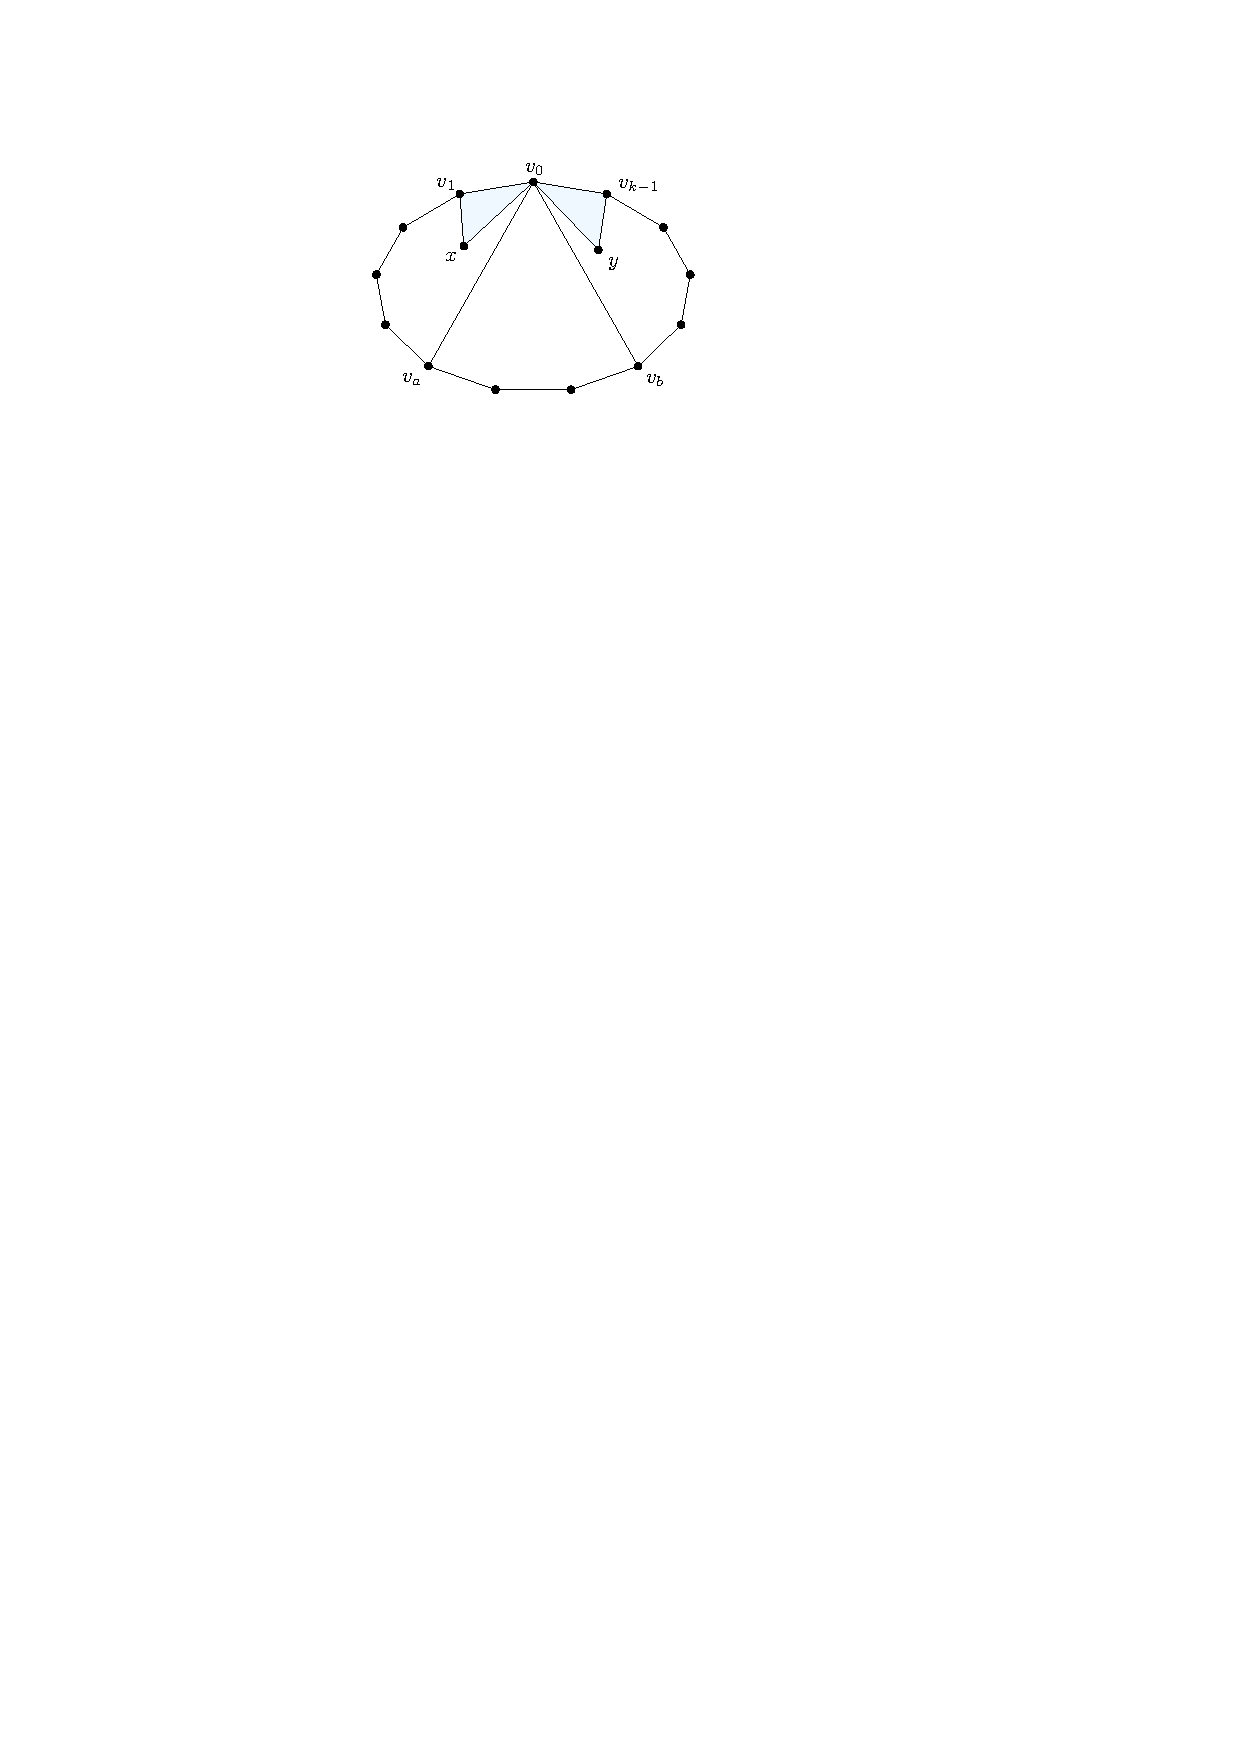
\includegraphics{figs/chord_incident}
%
%   \caption{The proof of \cref{chord_incident}}
%   \label{chord_incident_fig}
% \end{figure}
% \begin{proof}
%   Refer to \cref{chord_incident_fig}
%   Since $H$ is a near-triangulation its outer face is bounded by a cycle $v_0,\ldots,v_{k-1}$.  Let $a:=\min\{i\in\{2,\ldots,k-2\}:v_0v_i\in E(H)\}$ and $b:=\max\{i\in\{2,\ldots,k-2\}:v_0v_i\in E(H)\}$. (Possibly $a=b$, but both $a$ and $b$ are well-defined since $|N^+_H(v_0)|\ge 3$.)   Since $H$ is dom-minimal, the edge $v_0v_1$ is on the boundary of an inner face $v_0v_1x$ of $H$ where $x$ is an inner vertex of $H$.  Since $H$ is dom-minimal, the edge $v_{k-1}v_0$ is on the boundary of an inner face $v_{k-1}v_0y$ of $H$ where $y$ is an inner vertex of $H$.  Then $x$ is in the interior of the face of $H[B(H)]$ bounded by the cycle $v_0,v_1,\ldots,v_a$ and $y$ is in the interior of the face of $H[B(H)]$ bounded by the cycle $v_0,v_b,\ldots,v_{k-1}$.  Therefore, $x\neq y$ and $N^+_H(v_0)\supseteq\{x,y\}$ so $\deg^+_H(v_0)\ge 2$.
% \end{proof}
%
%
%
% Let $K_5^-$ be the complete graph on five vertices with one edge removed.
%
% \begin{lem}
%   Let $H$ be a near-triangulation with $\deg^+_H(z)\le 2$ for all $z\in B(H)$. If $\deg^+_H(v)=1$ for some $v\in B(H)$, then $H$ is isomorphic to $K_4$ or $K_5^-$.
% \end{lem}
%
% \begin{proof}
%   Since $H$ is dom-minimal each vertex in $B(H)$ has inner-degree at least $1$, by \cref{minimum_degree}.  Therefore the outer face of $H$ is a cycle with at least three vertices.  Let $u$ and $w$ be the two neighbours of $v$ on the outer face.  Since $H$ is dom-minimal, $H$ contains an inner face $vxu$ with $x\in I(H)$, by \cref{bad_edge}.  Since $H$ is dom-minimal, $H$ contains an inner face $wyv$ with $y\in I(H)$.  Since $\deg^+_H(v)=1$, $x=y$.  Since $H$ is dom-minimal $uw$ is an edge of $H$, by \cref{one_vertex}.  Therefore $uvx
% \end{proof}
%
% A subgraph $H'$ of a generalized near-triangulation $H$ is \defin{dom-preserving} if
% % every outer-domatic set $X\subseteq V(H')$ of $H'$ is an outer-domatic set of $H$.
%
% \begin{compactenum}[({DP}1)]
%   \item $B(H')\subseteq B(H)$; \label[dp]{smaller_boundary}
%   \item $N^+_{H'}(v)=N^+_H(v)$ for all $v\in B(H')$; \label[dp]{interior_preserving}
%   \item $I(H')=I(H)$; and \label[dp]{inner_neighbourhood_preserving}
%   \item $N_{H'}(v)=N_H(v)\cap V(H')$ for all $v\in I(H)$. \label[dp]{outer_neighbour_preserving}
% \end{compactenum}
%
% \begin{obs}
%   Let $H$ be a generalized near-triangulation, let $H'$ be a dom-preserving subgraph of $H$, and let $\Delta$ be a subset of $V(H')$ that dominates $I(H')$ in $H'$.  Then $\Delta$ dominates $I(H)$ in $H$.
% \end{obs}
%
% % \begin{proof}
% %   Each vertex $v\in I(H')$ is adjacent to some vertex $w\in \Delta$.  Since $N_{H'}(v)=N_H(v)$, $w\in\Delta\cap V(H')$, so $v$ is dominated by $\Delta\cap V(H')$.  Since this is true for each $v\in I(H)=I(H')$, $\Delta\cap V(H')$ dominates $I(H)$.
% % \end{proof}
%
% \begin{lem}\label{dom_minimal}
%   For any generalized near-triangulation $H$, there exists a dom-preserving subgraph $H'$ of $H$ that is dom-minimal.
% \end{lem}
%
% \begin{proof}
%   The proof is by induction on $|V(H)|+|E(H)|$.  If $H$ is already dom-minimal, then setting $H'=H$ satisfies the requirements of the lemma, so assume that $H$ is not dom-minimal.  It is straightforward to verify that the dom-preserving subgraph relationship is transitive, so if $H$ has a dom-preserving subgraph $H^*$ and $H^*$ has a dom-preserving subgraph $H'$ then $H'$ is a dom-preserving subgraph of $H$.  Therefore, it is sufficient to show the existence of a dom-preserving subgraph $H^*$ of $H$ with fewer edges or fewer vertices than $H$. Then the inductive hypothesis provides the desired dom-minimal dom-preserving subgraph $H'$ of $H$.
%
%   If $H$ contains a vertex $v\in B(H)$ with $\deg^+_H(v)=0$ then $H-v$ is a dom-preserving subgraph of $H$ with fewer vertices than $H$.  We now assume that $\deg^+_H(v)\ge 1$ for all $v\in B(H)$.  Since $H$ is not dom-minimal then $H$ contains a biconnected component $C$ that is not dom-minimal.
%   \begin{compactenum}
%     \item If there exists an edge $vw$ on the outer face of $C$ that is not incident to any inner face $vxw$ with $x\in I(C)$ then $B(H-vw)=B(H)$ and $I(H-vw)=I(H)$, and $H-vw$ is a is dom-preserving subgraph of $H$ that has fewer edges than $H$.
%
%     \item If there exists a vertex $v\in B(C)$ with $\deg^+_C(v)=0$ then $v$ is incident to an edge $vw$ that is on the outer face of $C$ and on the outer face of $H$. Since $\deg^+_C(v)=0$, $vw$ is not incident to any inner face $vwx$ with $x\in I(C)$ and we can proceed as in the previous case. \qedhere
%   \end{compactenum}
% \end{proof}
%


\bibliographystyle{plainurlnat}
\bibliography{main}

\appendix

\section{Sage Code}

\lstinputlisting[basicstyle=\ttfamily\scriptsize,language=Python]{cds.py}


\end{document}
